\documentclass[10pt]{article} % 10pt 字体大小,单栏布局
%\documentclass[10pt,journal]{IEEEtran}
\usepackage{ctex}          % 支持中文
\usepackage{cite}
\usepackage{amsmath,amssymb,amsfonts}
\usepackage{graphicx}
\usepackage{booktabs}
\usepackage{geometry}
\usepackage{subcaption} % 添加子图/子表格支持
\usepackage{setspace}
\usepackage{titlesec}
\usepackage{tikz}
\usepackage{float}
\usetikzlibrary{shapes.geometric, arrows, positioning}
\usepackage[ruled,vlined]{algorithm2e} % 算法格式支持

% 页面布局设置
\geometry{a4paper, left=0.5in, right=0.5in, top=0.5in, bottom=1in} % 减小页边距

% 标题格式设置
\titleformat{\section}{\large\bfseries}{\thesection\ }{0em}{} % 一级标题无点
\titleformat{\subsection}{\normalsize\bfseries}{\thesubsection\ }{0em}{} % 二级标题无点
\titleformat{\subsubsection}{\normalsize\bfseries}{\thesubsubsection\ }{0em}{} % 三级标题无点

% 行距设置
\setstretch{1.2} % 行距 1.2 倍

% 公式编号统一格式
\numberwithin{equation}{section}

\begin{document}

\title{\textbf{面向数据质量的清洗方法与下游聚类算法协同优化的自动化模型研究}}
\date{\today}
\maketitle

% 摘要部分
\noindent\textbf{\large 摘要} \\ 
在无监督学习任务中,数据质量问题(如错误值、缺失值与噪声)常显著影响聚类算法的性能。针对这一挑战,本文提出了一种协同优化方法,将数据清洗策略与聚类算法的组合纳入统一框架。通过构建综合得分体系,对多种清洗-聚类组合在不同数据集特征下的表现和适配性进行系统量化和广泛评估;同时,基于先验数据特征,采用多标签学习技术实现从“数据特征”到“优选方案子空间”的映射,显著减少搜索空间;在此基础上,我们设计了一种自动化管线优化模型,在保证聚类质量的前提下有效提升了时间效率。实验结果表明,本文方法在多个公开数据集上均表现出较高的聚类精度与显著的效率提升,验证了其在数据清洗与聚类协同优化中的实用性与鲁棒性。本研究为应对大规模、高噪声数据场景下的聚类问题提供了理论支持和实际解决方案。

\section{引言}
在许多实际应用场景中(例如医疗、金融以及工业物联网等领域),数据经常面临缺失值、错误值与噪声等质量问题。与分类或回归等有监督学习任务相比,聚类作为一种无监督学习方法对于数据分布的依赖性更为强烈,一旦数据中存在过多噪声或不确定性,就容易导致簇结构与真实分布出现显著偏离。这类偏离不仅影响聚类本身的准确性,也会对后续的模式挖掘和决策支持造成不可忽视的干扰。可见,在下游聚类任务中,数据质量对于结果的影响往往举足轻重。

为了减少噪声干扰与纠正错误数据,研究者们提出了多种数据清洗策略,包括缺失值填充、异常值检测与剔除、错误值纠正等。其核心目标在于“修复或减少数据中的噪声与错误”,以期在随后的分析过程中尽量保留准确可靠的分布结构。然而,清洗操作并不必然带来正向收益。有研究指出,过度严格的清洗可能修改或删除原本正确的数据;过于简单的填充策略则会扭曲原有分布特征,反而可能削弱聚类算法对关键信息的捕捉能力。在少量噪声的情形下,去除异常点确实能使 K-Means 算法获得更稳定的聚类效果,但若这些“异常点”恰恰是某些簇的重要特征,则对基于密度的聚类方法(如 DBSCAN算法)反而不利。由此可见,清洗方法与聚类算法之间存在紧密关联,如果仅从清洗或聚类单方面着手,往往难以兼顾双方需求。

现有研究通常在两条技术路线下分别进行:其一,机器学习视角侧重于改进聚类算法自身(例如 K-Means 的变体、层次聚类或密度聚类等);其二,数据质量视角主要针对如何提升数据完整性与准确度。然而,不同清洗策略会对数据分布带来不同程度的修正,而不同聚类算法又对噪声、缺失率等有着各自的敏感度,若只聚焦其中一端,难以获得全局最优的方案。因此,“清洗策略 + 聚类算法 + 超参数”一体的管线协同优化方案逐渐受到关注,但该管线的搜索空间常呈指数级增长,依赖人工穷举或简单试验往往难以在可接受的时间范围内完成。

为此,我们尝试在“数据质量(数据清洗理论)”与“自动化机器学习(AutoML)”两大领域之间建立桥梁,引入自动化聚类模型(基于AutoML的思路)来缩减庞大的管线搜索开销并兼顾聚类质量。当前大部分 AutoML 研究主要集中在有监督学习任务(如分类和回归)的模型选择与超参数优化上,对无监督学习——尤其是“聚类 + 清洗”这种协同自动化的探索仍较为有限。因此,本研究将多种清洗方法、聚类算法及其参数一并纳入搜索空间,通过学习模型捕捉“数据特征与优选方案组合”之间的映射关系。当面对新的数据集及其特征时,系统能够自动推荐若干优选的清洗-聚类-参数组合,既能减少冗余探索,又能提升聚类效果的稳定性和准确性。

在无监督学习场景下,协同优化的自动化框架具有显著的潜力。聚类算法在产业界和学术界有着广泛的应用场景,而大多数真实世界的数据通常都存在一定的质量问题。因此,如果能够实现对数据质量的适配清洗与高效聚类的有机结合,将大大拓宽聚类技术的应用范围,促进其在更多领域的落地。针对这一尚未得到充分探索的方向,本研究提出了一个面向数据质量的清洗与聚类协同优化的自动化模型。这一模型不仅为学术研究提供了新的思路,也有望在实际应用中发挥重要作用。

\textbf{贡献}。我们针对“数据清洗与下游聚类协同优化”这一交叉研究领域,围绕算法性能与自动化效率,总结如下方面的贡献:
\begin{enumerate}
    \item \textbf{系统评估多种清洗-聚类组合的有效性与局限性}  

    我们基于 40 个具备多元质量问题的公开数据集,深入研究了 3 种清洗策略与 6 种聚类算法的交互关系,并针对不同错误率、噪声水平及数据规模的多场景进行实验测试。通过大量实证结果,量化了清洗方法与聚类算法之间的适配度,并揭示了特定组合在极端环境(如高维度、高错误率数据)下可能产生的极端现象及风险。这些结论为后续的清洗-聚类管线设计提供了可操作的参考依据,丰富了现有文献在无监督学习场景下对数据质量处理方法的系统性比较。

    \item \textbf{提出基于管线思维的清洗与聚类协同优化框架}  

    我们将“数据清洗策略 + 聚类算法 + 超参数”视作一个整体管线(Pipeline),并结合实验结果总结出在不同场景下的优先组合与适配性建议。该框架帮助研究者在设计无监督学习流程时,能同时考虑数据质量和算法性能,避免了只聚焦某一端而造成的局限性。

    \item \textbf{构建并验证了自动化管线优化模型,显著提升效率与性能}  

    在深入理解清洗与聚类之间协同关系的基础上,我们进一步设计了一种自动化管线模型:该模型能够根据数据集特征快速筛选可能的最优清洗-聚类组合,大幅削减搜索空间。与传统手动调参或穷举策略相比,自动化模型在效率指标上展现出显著优势,同时在多数数据集上保持了与完整搜索接近的聚类效果。我们以损失率(Loss Rate)和综合加速比(Acceleration Ratio)等指标量化了该模型在平衡聚类质量与运行时间方面的成效,为未来在大规模和多样化数据场景下的应用提供了可迁移的实践路径。

\end{enumerate}

%---------------------------------
% 第二章:相关工作
%---------------------------------

\section{相关工作}\label{sec:related_work}

当前针对数据清洗模型与聚类算法的研究,主要集中在以下三个方向:\textbf{(1) 机器学习视角下的聚类算法改进;(2) 数据质量视角下的清洗策略优化;(3) 无监督场景中的自动化机器学习探索}。本节将对相关工作进行梳理,并指出与本研究的区别。

\subsection{机器学习视角:聚类算法的改进}
从机器学习的角度,研究者更多关注聚类算法本身的改进和变体设计。例如,K-Means 在初始中心选择、迭代更新策略等方面衍生了多种增强方法,以提升收敛速度或降低局部最优的风险;层次聚类与图聚类则在相似度度量和聚类结构可视化方面提出了新的思路。不过,这些研究通常默认数据预处理已经完成,或在简单清洗之后才进行聚类算法的优化,往往没有深入讨论不同清洗策略对数据分布和聚类效果的潜在影响。

\subsection{数据质量视角:清洗策略及其影响}
从数据质量视角出发,学者们在缺失值填充、异常值检测与错误值纠正等方面做了大量探索。常见方法包括基于统计或回归模型的缺失值插补,基于密度或距离的异常值检测等。然而,不同清洗策略对下游聚类效果的具体影响仍缺乏系统验证,大多数工作只选择单一或少数聚类算法进行测试,对不同聚类方法在噪声和缺失率方面的差异需求尚未形成全面比较。

\subsection{自动化机器学习:无监督场景的探索}
AutoML 在有监督学习(分类与回归)方面已经取得了显著进展,如自动模型选择和超参数搜索等~\cite{ref13, ref14}。然而,对于无监督学习,尤其是“聚类 + 清洗”的联合自动化仍处于相对初步的探索阶段。现有少数工作关注自动确定聚类数目或部分预处理自动化,但尚未建立起“清洗策略 + 聚类算法 + 超参数”的综合管线搜索体系。

\subsection{与本研究的差异}
综合上述三个方向,可以发现现有研究在“清洗-聚类”协同优化方面尚存在以下不足:
\begin{itemize}
    \item \textbf{缺乏清洗与聚类交互影响的系统性评估}:当前研究多侧重于独立优化聚类算法或改进清洗策略,缺乏对两者交互影响的系统性分析,特别是在多场景、多数据特征下的验证。
    \item \textbf{缺乏统一的自动化管线优化框架}:现有方法通常通过手动配置或依赖单一预处理方案来调整清洗与聚类过程,缺少能够动态适配不同数据特征的端到端管线式优化框架。
    \item \textbf{高效搜索机制的缺失}:面对清洗策略、聚类算法及其超参数构成的庞大搜索空间,现有方法在效率和性能平衡方面仍存短板,难以满足实际应用中对快速与高质量结果的需求。
\end{itemize}

针对上述问题,本文提出了一种自动化管线优化模型,将清洗策略、聚类算法及超参数统一纳入动态优化框架。通过结合数据特征和实验分析,我们的模型能够高效捕捉最优组合方案,并在多种场景中验证了其性能优势和适配性。与现有研究相比,本研究的自动化管线框架从全局角度实现了数据清洗与聚类算法的协同优化,为无监督学习提供了新的研究方向与实践路径。

%---------------------------------
% 第三章:问题和模型定义
%---------------------------------
\section{问题和模型定义}
\label{sec:problem-and-model}

在各种实际应用(如医疗、金融以及工业物联网等)中,数据由于错误值、缺失值及噪声等问题而呈现出多元的质量特征。如果仅依赖单一的预处理或聚类方式,往往难以兼顾不同场景下的精度需求与时间成本。为在理论与应用中更好地理解并解决“数据清洗与聚类算法”的协同优化,本节将依次介绍相关概念、系统化的评价方法,以及应的映射模型,最后给出核心研究问题的形式化描述。

\subsection{核心概念与变量定义}
\label{subsec:core-concepts}

令 \(D\) 表示待处理的数据集,其中可能同时存在错误值(Error)、缺失值(Missing)以及噪声(Noise)等质量问题。为了刻画这些问题与数据规模的差异,定义\textbf{特征向量}
\begin{equation}\label{eq:xD}
  \mathbf{x}(D) 
  \;=\; 
  \bigl(\mathrm{ErrorRate}(D),\; \mathrm{MissingRate}(D),\; \mathrm{NoiseRate}(D),\; m,\; n\bigr),
\end{equation}
其中 \(\mathrm{ErrorRate}(D)\)、\(\mathrm{MissingRate}(D)\) 与 \(\mathrm{NoiseRate}(D)\) 分别表示数据集中错误值、缺失值以及噪声的相对比例,\(m\) 和 \(n\) 分别为数据的特征维度与样本规模。该向量不仅能在不同场景下进行横向对比,也为后续的映射模型提供了可学习的输入特征。

在数据清洗与聚类算法的设定中,记 \(\mathcal{C}\) 为数据清洗方法的集合(如缺失值插补、异常值剔除、错误值纠正等),\(\mathcal{H}\) 为聚类算法的集合(如 K-Means、DBSCAN、层次聚类等),\(\mathcal{P}\) 为聚类算法的超参数空间。将一个具体的清洗方法 \(c\)、聚类算法 \(h\) 及其超参数 \(\boldsymbol{\theta}\) 组合成\textbf{清洗-聚类策略}
\begin{equation}\label{eq:omega}
  \omega 
  \;=\; 
  \bigl(c,\; h,\; \boldsymbol{\theta}\bigr),
\end{equation}
所有可行策略的笛卡尔积构成初始搜索空间
\begin{equation}\label{eq:Omega}
  \Omega 
  \;=\; 
  \mathcal{C} \;\times\; \mathcal{H} \;\times\; \mathcal{P}.
\end{equation}
在实际应用中,\(\Omega\) 的规模常随数据清洗或聚类算法的多样性呈现出指数级增长,因此对其进行穷举评估常常带来巨大的时间与计算负担。

\subsection{评价系统与最优方案}
\label{subsec:evaluation-system}

为衡量任意策略 \(\omega \in \Omega\) 在数据集 \(D\) 上的聚类质量,通常采用若干无监督指标加以综合。本文主要采用 Davie-Bouldin(DB)指数与轮廓系数(Silhouette)两类典型指标,并将它们线性组合为\textbf{综合得分}。

首先,对于算法划分出的 \(K\) 个簇,DB 指数通过考察簇内紧凑度与簇间分离度来衡量聚类效果,具体定义为
\begin{equation}\label{eq:db-score}
  DB(D,\omega)
  \;=\;
  \frac{1}{K}\sum_{i=1}^{K}
  \max_{j\neq i}
  \Bigl(\frac{S_i + S_j}{d_{ij}}\Bigr),
\end{equation}
其中 \(S_i\) 为第 \(i\) 个簇的平均离散度,\(d_{ij}\) 为簇 \(i\) 与簇 \(j\) 的中心距离,数值越低表示聚类效果越理想。

其次,轮廓系数(Silhouette Coefficient)量化了每个样本点 \(x\) 在其所属簇内的凝聚度以及跟最近邻簇的分离度,定义为:
\begin{equation}\label{eq:silhouette}
  \mathrm{Sil}(x)
  \;=\;
  \frac{b(x) - a(x)}{\max\bigl\{a(x),\,b(x)\bigr\}},
\end{equation}
其中 \(a(x)\) 表示 \(x\) 与同簇内其他样本的平均距离,\(b(x)\) 表示 \(x\) 到最近邻簇内样本的平均距离。总体轮廓系数为所有样本轮廓系数的平均值:
\begin{equation}\label{eq:average-silhouette}
  \mathrm{Sil}(D,\omega)
  \;=\;
  \frac{1}{n} \sum_{x \in D} \mathrm{Sil}(x),
\end{equation}
其中 \(n\) 为数据集 \(D\) 中样本的总数。平均轮廓系数越高,表示聚类划分越合理。

结合 DB 指数与轮廓系数,可定义\textbf{综合得分},以量化清洗-聚类策略的整体效果:
\begin{equation}\label{eq:S-score}
  S(D,\omega)
  \;=\;
  \alpha \cdot \bigl[-\,DB(D,\omega)\bigr]
  \;+\;
  \beta \cdot \mathrm{Sil}(D,\omega),
\end{equation}
其中 \(\alpha,\beta > 0\) 为可调权重,\(\bigl[-\,DB(D,\omega)\bigr]\) 项强调 DB 指数越低越好,便于与轮廓系数在同一方向上加和。通过综合得分 \(S(D,\omega)\),本文能够系统评估不同清洗-聚类策略组合在特定数据集上的性能,并为优选方案提供直观依据。

当我们仅从聚类精度角度出发,给定 \(D\) 的最优策略可表示为
\begin{equation}\label{eq:best strategy}
  \omega^*(D)
  = \arg\max_{\omega \,\in\, \Omega} S(D,\omega).
\end{equation}
然而,若要在全量空间 \(\Omega\) 上评估每个策略 \(\omega\),往往需要花费大量计算时间。为此,我们将定义一个\textbf{优化子空间} \(\Omega'(D)\subseteq \Omega\),仅在其中执行评估,以缓解时间消耗。假设评估单个策略的耗时记为 \(T(D,\omega)\),则
\begin{equation}\label{eq:T-original}
  T_{\text{original}}(D)
  \;=\;
  \sum_{\omega \,\in\, \Omega} \, T(D,\omega)
\quad\text{与}\quad
  T_{\text{reduced}}(D)
  \;=\;
  \sum_{\omega \,\in\, \Omega'(D)} \, T(D,\omega)
\end{equation}
分别表示完整搜索与缩减搜索的总耗时。若 \(\Omega'(D)\) 能在\textbf{保证聚类质量}的情况下大幅减少评估开销,即可平衡精度与效率。为度量这两方面的综合效果,引入\textbf{损失率}与\textbf{综合加速比}。

\subsubsection*{损失率与综合加速比}
若令 \(\bar{S}(\Omega)\) 表示在完整搜索 \(\Omega\) 上得到的平均得分,\(\bar{S}(\Omega'(D))\) 表示在优选子空间 \(\Omega'(D)\) 中的平均得分,则可定义
\begin{equation}\label{eq:loss-rate}
  \eta(D)
  =
  1 \;-\;
  \frac{\bar{S}(\Omega'(D))}{\bar{S}(\Omega)},
\end{equation}
作为\textbf{损失率},反映缩减搜索后对聚类质量的平均影响;值越接近 0,表示压缩空间后性能损失越小。此外,记
\begin{equation}\label{eq:acc-ratio}
  \mathcal{A}(D)
  =
  \Bigl(1 - \eta(D)\Bigr)
  \;\times\;
  \frac{T_{\text{original}}(D)}{T_{\text{reduced}}(D)},
\end{equation}
作为\textbf{综合加速比},数值越大意味着在质量损失可控的前提下获得了更显著的搜索加速效果。

\subsection{从数据特征到优选方案的映射}
\label{subsec:mapping-model}

在应用场景中,不同数据集 \(D\) 往往拥有差异明显的特征向量 \(\mathbf{x}(D)\),如错误率、缺失率、噪声率、样本规模等(参考式~\eqref{eq:xD})。这些特征会显著影响“数据清洗 + 聚类算法”组合的表现,使得某些策略更契合特定类型的数据分布。若能提前根据 \(\mathbf{x}(D)\) 预测哪些组合最可能获得较高综合分数 \(S(D,\omega)\),就可减少对大规模搜索空间 \(\Omega\) 的穷举评估,进而大幅缩减时间成本。

为此,本文引入一个映射函数
\begin{equation}\label{eq:Omega-prime}
  G:\, \mathbf{x}(D)\,\mapsto\, \Omega'(D),
\end{equation}
其中 \(\Omega'(D)\subseteq \Omega\) 为一个规模较小的\textbf{优选子空间}。通过在先验数据集上积累“数据特征—策略表现”的关联信息,便可利用机器学习或统计方法(例如多标签分类)训练出映射 \(G\),使其在新数据集上快速推荐表现优良的候选组合,从而避免对完整空间 \(\Omega\) 的重复尝试。后续章节将结合实例场景和模型设计,详细说明如何构建并验证该映射。

\subsection{核心问题的形式化定义}
\label{subsec:problem-formalization}

在介绍了数据集特征、清洗-聚类策略与映射函数等概念后,现对本文的核心研究任务做形式化总结。具体而言,本研究聚焦以下三个关键问题:

\paragraph{(1) 定量评估与比较不同清洗-聚类组合的协同表现}
在初始搜索空间 \(\Omega\) 中,每个策略 \(\omega\) 都可根据综合得分 \(S(D,\omega)\) 进行排名。如何通过该排名定量分析与比较不同组合在\textbf{适配性}和\textbf{协同优化}方面的表现,进而识别出在给定数据集 \(D\) 上效果最为突出的组合?这一过程需要关注数据质量特征对综合得分的影响机理,并结合最优策略 \(\omega^*(D)\) 或排名靠前的若干策略作综合评判。

\paragraph{(2) 寻找并建立数据特征到优选方案集合的映射模型}
当数据集特征差异较大时,最优或近优的组合往往随之发生变化,难以通过固定规则一概而论。如何\textbf{基于数据特征} \(\mathbf{x}(D)\) 来\textbf{自动}或\textbf{半自动}地推荐一个优选子空间 \(\Omega'(D)\),从而在不显著损失聚类质量的情况下减少搜索规模?为解决这一问题,需要构建映射函数
\[
  G:\,\mathbf{x}(D)\,\mapsto\,\Omega'(D),
\]
并在先验数据集上学习和验证该函数的可靠性。

\paragraph{(3) 建立自动化模型以在有限时间内找到接近最优的方案,并尽量提高综合加速比}
若直接对 \(\Omega\) 进行完整搜索,将面临极高的时间成本。因而,需要设计一个\textbf{自动化}流程:在给定 \(\mathbf{x}(D)\) 之后,仅在子空间 \(\Omega'(D)\) 进行快速评估,找到
\begin{equation}\label{eq:local best strategy}
  \hat{\omega}(D) 
  = 
  \arg\max_{\omega \,\in\,\Omega'(D)} \, S(D,\omega).
\end{equation}
同时,引入\textbf{损失率} \(\eta(D)\) 和\textbf{综合加速比} \(\mathcal{A}(D)\)(参考式~\eqref{eq:loss-rate} 与~\eqref{eq:acc-ratio}),量化压缩搜索空间带来的精度损失与效率提升。在\textbf{有限时间}内实现较低损失率与较高加速比,为实际部署提供可行的协同优化方案。

基于上述三方面的研究重点,本文将从实验与算法设计两个角度展开:首先在多个具有噪声、缺失或错误值的问题数据集中,系统验证和评估不同清洗-聚类组合的表现和适配性;然后以多标签学习或自动化搜索策略为基础,搭建映射机制与自动化管线,力图在有限时间内逼近最优聚类效果并兼顾运行效率。后续章节将对具体的模型结构、实验步骤及结果进行详细阐述。

%---------------------------------
% 第四章:自动化聚类方法
%---------------------------------

\section{自动化聚类方法}
\label{sec:autoML}

为进一步提高清洗-聚类策略的搜索效率,本节将在第~\ref{sec:problem-and-model} 节所述概念的基础上,介绍将数据划分为先验数据与测试数据、使用多标签学习构建映射函数,以及最终实现自动化聚类优化流程的整体方法。该方法旨在通过离线阶段积累的先验知识,缩减在线搜索空间,从而在\textbf{较短时间}内找到\textbf{接近最优}的清洗-聚类组合并兼顾评估效率。
以下是本章节所定义的符号与描述:

\begin{table}[ht]
\centering
\small % 设置表格字体为0.8倍
\renewcommand{\arraystretch}{1.1} % 适当调整行距
\label{tab:symbols-advanced}
\begin{tabular}{ll}
\toprule
\textbf{符号} & \textbf{描述} \\
\midrule
$D_{\text{train}}$ & 先验数据集(训练集),用于离线评估和学习先验知识 \\
$D_{\text{test}}$ & 测试数据集,用于实际部署和快速优化 \\
$K$ & Top-K 大小,表示在先验阶段选取的前 $K$ 个最优方案 \\
$\mathbf{M}^{(i)}$ & 数据集 $D^{(i)}$ 的 Top-K 策略矩阵 \\
$\ell$ & 标签,表示某一优选方案的标识符 \\
$\mathcal{L}$ & 标签空间,包含所有优选方案的标签集合 \\
$\mathbf{L}^{(i)}$ & 数据集 $D^{(i)}$ 对应的多标签集合 \\
$\mathcal{M}$ & 训练集,包含所有先验数据的特征与标签集合 \\
$\mathcal{F}$ & 多标签分类器,用于预测优选方案标签 \\
$q^{(j)}$ & 标签 $\ell_{\omega^{(j)}}$ 为优选方案的概率 \\
$r$ & 预测阶段保留的最高优选标签数 \\
$\mathbf{L}'$ & 预测阶段保留的最高优选标签集合 \\
$\Omega'(D)$ & 数据集 $D$ 的优选子空间,$\Omega'(D) \subseteq \Omega$ \\
$G$ & 映射函数,将数据集特征向量映射到优选子空间 \\
$\hat{\omega}$ & 最优方案,即在 $\Omega'(D_{\text{test}})$ 中得分最高的组合 \\
\bottomrule
\end{tabular}
\caption{符号与描述}
\end{table}
\subsection{先验数据与多标签映射策略}
\label{sec:prior-data-mapping}


在实际应用中,通常可以从历史任务中获取大量已处理或部分标注的数据集,这些可视为\textbf{先验数据}(离线学习)。当面对新任务时,由于需要在较短时间内完成聚类策略的优选与评估,此时的新数据集则称为\textbf{测试数据}(在线应用)。通过在先验数据上深入探索并记录“数据特征—策略表现”的关联信息,就能在测试数据上显著减少不必要的搜索开销,从而提升整体效率。

\subsubsection{先验数据与测试数据的划分}
\label{subsec:dataset-split}

为便于在实际部署时利用先验知识,本研究将原有数据资源分为以下两类:
\begin{itemize}
    \item \textbf{先验数据集} $D_{\text{train}}$:由多个历史数据集组成,记为 ${D^{(1)}, D^{(2)}, \dots, D^{(N)}}$。在离线阶段(训练阶段),这些数据用于对搜索空间 $\Omega$ 进行大范围或抽样评估,以收集足够的策略得分信息,为后续自动化优化提供参考。
    \item \textbf{测试数据集} $D_{\text{test}}$:代表实际部署时面临的新数据,需要在线快速找到近优的清洗-聚类组合。此时可借助先验阶段所学知识,显著减少搜索规模并降低评估时间。
\end{itemize}

在离线评估过程中,若对每个先验数据集 $D^{(i)}$ 遍历或随机抽样若干清洗-聚类策略 $\omega \in \Omega$,便可计算各自方案的综合得分 $S(D^{(i)}, \omega)$。为高效记录在 $D^{(i)}$ 上表现最好的候选策略集,我们定义一个\textbf{Top-K 方案矩阵}(式~\eqref{eq:topK-matrix}),记为 $\mathbf{M}^{(i)}$,其中每一行是一个评分 $S_j$ 较高的策略组合 $\omega_j^{(i)}=(c_j,h_j,\boldsymbol{\theta}_j)$。该矩阵按照 $S_j$ 降序排列,用于在后续多标签学习中标识“优选”方案。

\begin{equation}\label{eq:topK-matrix}
\mathbf{M}^{(i)} 
= 
\begin{pmatrix}
c_1 & h_1 & \boldsymbol{\theta}_1 & S_1 \\
\vdots & \vdots & \vdots & \vdots \\
c_K & h_K & \boldsymbol{\theta}_K & S_K
\end{pmatrix}.
\end{equation}

\subsubsection{多标签学习与映射函数构建}
\label{subsec:multi-label}

在离线阶段,除了得到各数据集 $D^{(i)}$ 的 Top-K 策略外,还要提取其特征向量 $\mathbf{x}(D^{(i)})$。通过\textbf{多标签学习}的方法,可将“数据特征”与“优选策略集合”关联起来,从而在面对新数据集 $D_{\text{test}}$ 时,根据其特征向量 $\mathbf{x}(D_{\text{test}})$ 预测出最优或近优的策略子空间 $\Omega'(D_{\text{test}})$。

\paragraph{标签空间与多标签构造}  
在离线阶段,为了构建从数据特征到优选方案的映射模型,需引入\textbf{标签空间}的概念。首先,将所有先验数据集中出现过的“优选策略”记录下来,表示为:
\[
\{\omega^{(1)}, \omega^{(2)}, \ldots, \omega^{(m)}\},
\]
并为每个优选策略 $\omega^{(j)}$ 赋予唯一标签 $\ell_{\omega^{(j)}}$,从而形成一个离散的\textbf{标签空间}:
\begin{equation}\label{eq:label-space}
\mathcal{L}
= \{\ell_{\omega^{(1)}}, \ell_{\omega^{(2)}}, \ldots, \ell_{\omega^{(m)}}\}.
\end{equation}

对于某个先验数据集 $D^{(i)}$,其 Top-K 组合 $\mathbf{M}^{(i)}$(式~\eqref{eq:topK-matrix})中每个策略都可视为一个“正”标签。这些标签的集合定义为:
\begin{equation}\label{eq:label-space-for-D}
\mathbf{L}^{(i)}
= \{\ell_{\omega_1^{(i)}}, \ell_{\omega_2^{(i)}}, \ldots, \ell_{\omega_K^{(i)}}\}.
\end{equation}

结合数据集的特征向量 $\mathbf{x}(D^{(i)})$,可构造出多标签训练样本:
\[
\bigl(\mathbf{x}(D^{(i)}), \mathbf{L}^{(i)}\bigr).
\]
最终,所有先验数据集的多标签样本汇总成多标签训练集 $\mathcal{M}$:
\begin{equation}\label{eq:training-set}
\mathcal{M}
= \bigl\{\bigl(\mathbf{x}(D^{(1)}), \mathbf{L}^{(1)}\bigr), \ldots, \bigl(\mathbf{x}(D^{(N)}), \mathbf{L}^{(N)}\bigr)\bigr\}.
\end{equation}

\paragraph{分类器训练与映射生成}  
在完成多标签训练集 $\mathcal{M}$ 的构造后,下一步是利用该训练集对多标签分类器 $\mathcal{F}$ 进行训练。分类器的目标是学习数据特征 $\mathbf{x}(D)$ 与优选策略标签 $\mathcal{L}$ 之间的关联关系。

具体而言,分类器 $\mathcal{F}$ 的输出为每个标签 $\ell_{\omega^{(j)}}$ 的置信度 $q^{(j)} \in [0,1]$。对任意给定的新数据集 $D_{\text{test}}$,输入其特征向量 $\mathbf{x}(D_{\text{test}})$ 后,分类器将返回以下形式的预测结果:
\begin{equation}\label{eq:classifier}
\mathcal{F}\bigl(\mathbf{x}(D_{\text{test}})\bigr)
= \bigl\{(\ell_{\omega^{(1)}}, q^{(1)}), (\ell_{\omega^{(2)}}, q^{(2)}), \ldots, (\ell_{\omega^{(m)}}, q^{(m)})\bigr\},
\end{equation}
其中 $q^{(j)}$ 表示数据集 $D_{\text{test}}$ 在优选策略 $\omega^{(j)}$ 下的置信度。

为减少评估成本,仅选取置信度最高的 $r$ 个标签,构成优选标签集合:
\begin{equation}\label{eq:predicted-label-space}
\mathbf{L}' = \bigl\{\ell_{\omega^{(j)}} \,\mid\, q^{(j)} \text{ 属于前}r\text{大值}\bigr\}.
\end{equation}
将这些标签映射回对应的清洗-聚类策略,得到优化后的\textbf{优选子空间}:
\begin{equation}\label{eq:optimized-space}
\Omega'(D_{\text{test}})
= \bigl\{\omega^{(j)} \,\mid\, \ell_{\omega^{(j)}} \in \mathbf{L}'\bigr\}.
\end{equation}

此时,优选子空间 $\Omega'(D_{\text{test}})$ 通常远小于原始搜索空间 $\Omega$,从而在减少计算成本的同时,保持较高的聚类质量。最终,该映射过程可表示为:
\begin{equation}\label{eq:mapping-function}
G\bigl(\mathbf{x}(D)\bigr) = \Omega'(D).
\end{equation}

\subsection{自动化聚类优化流程}
\label{sec:autocluster-process}

在第~\ref{sec:prior-data-mapping} 节中,我们介绍了如何利用先验数据构建多标签映射策略,以学习数据特征 $\mathbf{x}(D)$ 与优选方案子空间 $\Omega'(D)$ 之间的映射关系。基于这一映射,本节将进一步探讨其在\textbf{自动化聚类优化流程}中的应用,重点分析如何利用该知识在新数据上高效筛选清洗-聚类组合,从而减少搜索空间并提高优化效率。

\begin{figure}[htbp]
  \centering
  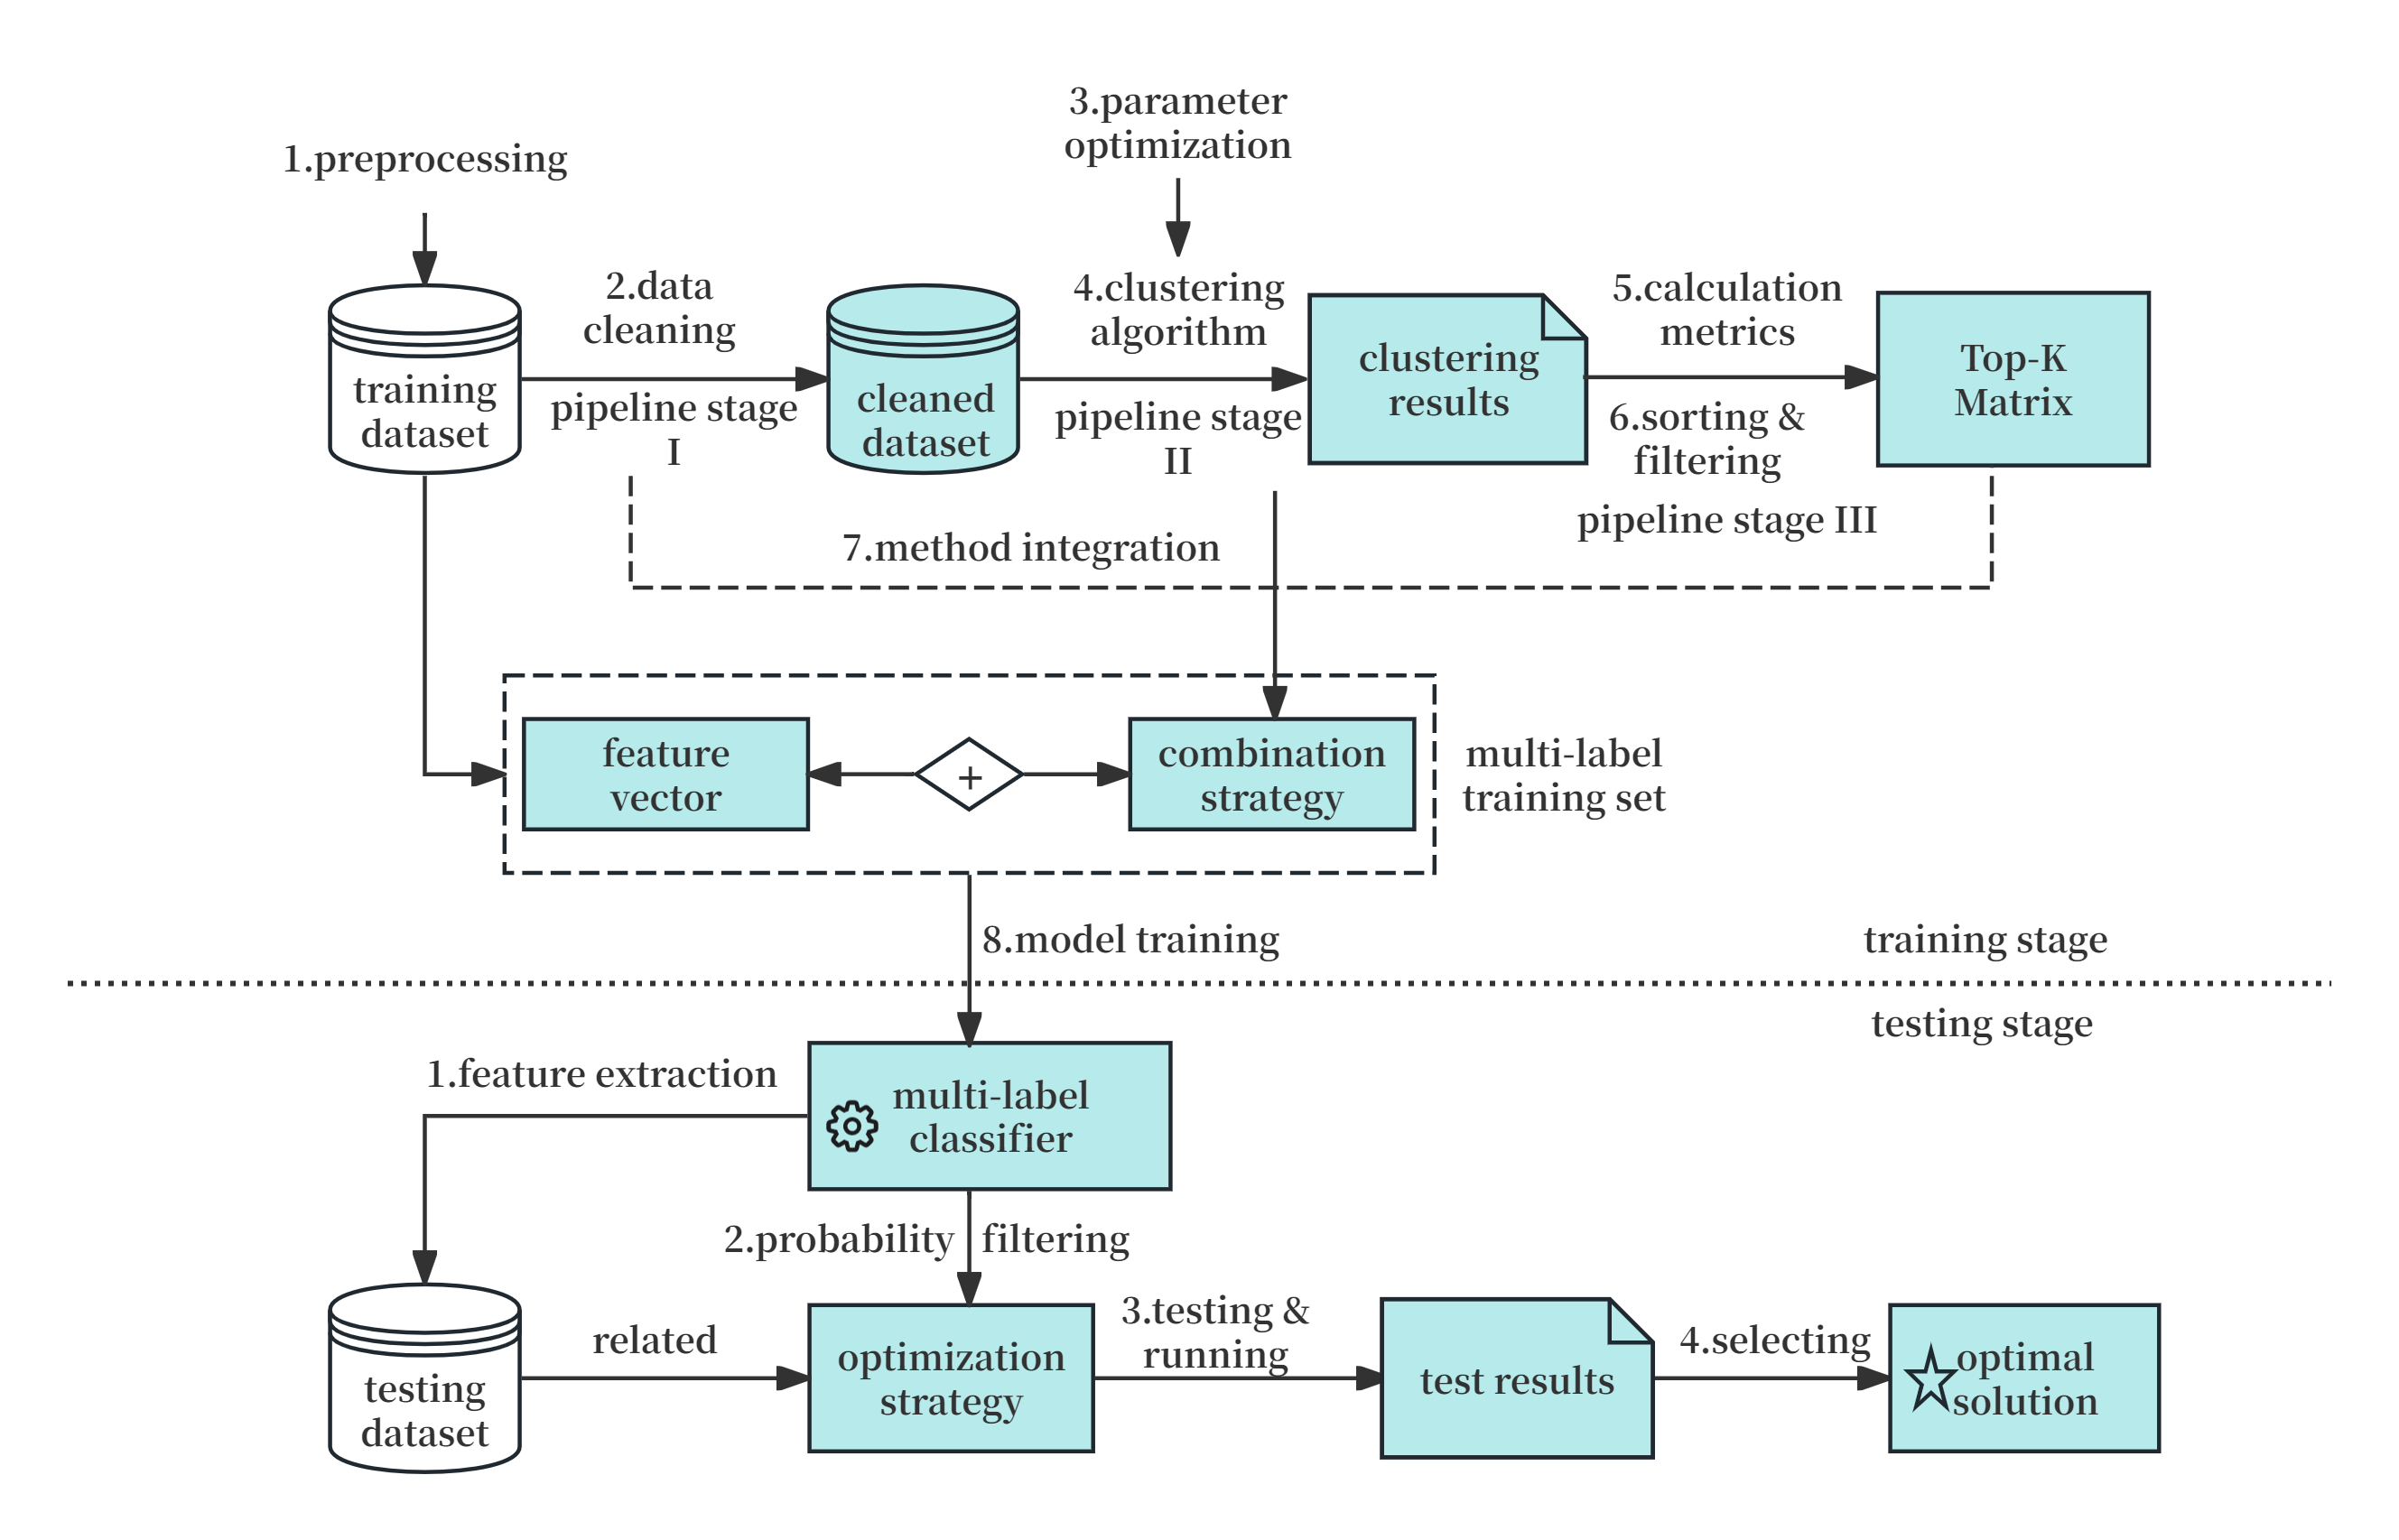
\includegraphics[width=0.85\linewidth]{figures/autocluster_workflow.png}
  \caption{自动化聚类优化流程示意图}
  \label{fig:autocluster-workflow}
\end{figure}

如图~\ref{fig:autocluster-workflow} 所示,自动化优化流程主要包括\textbf{离线知识积累}(训练阶段)和\textbf{在线优化}(测试阶段)两个核心环节: \begin{enumerate} \item \textbf{训练阶段(离线学习)}:基于先验数据集 $D_{\text{train}}$,计算不同数据特征与清洗-聚类策略的匹配程度,并训练多标签分类器 $\mathcal{F}$,从而建立数据特征到优选方案子空间的映射 $G(\mathbf{x}(D))$。 \item \textbf{测试阶段(在线优化)}:面对新的数据集 $D_{\text{test}}$,利用训练阶段学习到的映射 $G(\mathbf{x}(D_{\text{test}}))$,快速筛选搜索空间 $\Omega$ 中的候选策略子集 $\Omega'(D_{\text{test}})$,避免全量穷举,从而在较短时间内获取高质量的清洗-聚类方案。 \end{enumerate}

在接下来的小节中,我们将详细介绍两个阶段的具体实现,并给出关键算法的伪代码。

\subsubsection{训练阶段:离线知识积累}
训练阶段的目标是基于先验数据集 \(D_{\text{train}}\) 生成多标签训练集并学习多标签分类器。算法伪代码如算法~\ref{alg:train-phase} 所示。

\begin{algorithm}[H]
\caption{离线训练阶段:生成训练数据与训练多标签分类器}
\label{alg:train-phase}
\KwIn{
    先验数据集 $D_{\text{train}}=\{D^{(1)},\dots,D^{(N)}\}$;\\
    搜索空间 $\Omega$;\\
    Top-K 大小 $K$。
}
\KwOut{多标签分类器 $\mathcal{F}$}

\SetKwFunction{GenerateTrainingData}{GenerateTrainingData}
\SetKwFunction{TrainClassifier}{TrainClassifier}

$\mathcal{M} \leftarrow \GenerateTrainingData(D_{\text{train}}, \Omega, K)$\;
$\mathcal{F} \leftarrow \TrainClassifier(\mathcal{M})$\;
\KwRet{$\mathcal{F}$}

\bigskip

\SetKwProg{Fn}{Function}{:}{}
\Fn{\GenerateTrainingData{$D_{\text{train}}, \Omega, K$}}{
  $\mathcal{M} \leftarrow \emptyset$\;
  \For{$i \leftarrow 1$ \KwTo $|D_{\text{train}}|$}{
    \ForEach{$\omega \in \Omega$ \textbf{(或采样自 $\Omega$)}}{
      计算 $S(D^{(i)}, \omega)$\;
    }
    选出 Top-K 策略 $\mathbf{M}^{(i)} = \{\omega_1^{(i)}, \dots, \omega_K^{(i)}\}$ 按得分降序\;
    映射为多标签集合 $\mathbf{L}^{(i)} = \{\ell_{\omega_1^{(i)}}, \dots, \ell_{\omega_K^{(i)}}\}$\;
    $\mathcal{M} \leftarrow \mathcal{M} \cup \{(\mathbf{x}(D^{(i)}), \mathbf{L}^{(i)})\}$\;
  }
  \KwRet{$\mathcal{M}$}
}

\Fn{\TrainClassifier{$\mathcal{M}$}}{
  \tcp{可根据具体多标签算法实现}
  训练多标签分类器 $\mathcal{F}$\;
  \KwRet{$\mathcal{F}$}
}
\end{algorithm}

\subsubsection{测试阶段:在线预测与最优方案搜索}
测试阶段在新数据集 \(D_{\text{test}}\) 上应用训练好的分类器,快速锁定优选子空间并搜索最优策略。伪代码如算法~\ref{alg:test-phase} 所示。

\begin{algorithm}[H]
\caption{测试阶段:寻找最优方案 \(\hat{\omega}\)}
\label{alg:test-phase}
\KwIn{
    测试数据集 $D_{\text{test}}$;\\
    多标签分类器 $\mathcal{F}$;\\
    搜索空间 $\Omega$;\\
    保留标签数 $r$。
}
\KwOut{最优方案 $\hat{\omega}$}

计算 $\mathbf{x}(D_{\text{test}})$\;
$\mathbf{L}' \leftarrow \{\}$\;
\ForEach{$\ell \in \mathcal{L}$}{
  $q_{\ell} \leftarrow \text{置信度}(\mathcal{F}, \mathbf{x}(D_{\text{test}}), \ell)$\;
  $\mathbf{L}' \leftarrow \mathbf{L}' \cup \{(\ell, q_{\ell})\}$\;
}
选取置信度最高的 $r$ 个标签 $\mathbf{L}'_{\mathrm{top}}$\;
映射回优选子空间 $\Omega'(D_{\text{test}})$\;
\ForEach{$\omega \in \Omega'(D_{\text{test}})$}{
    计算 $S(D_{\text{test}}, \omega)$ \tcp*{计算综合得分}
}
$\hat{\omega} \leftarrow \arg\max_{\omega \in \Omega'(D_{\text{test}})}S(D_{\text{test}}, \omega)$\;
\KwRet{$\hat{\omega}$}
\end{algorithm}

\subsection{小结}
本节系统介绍了自动化聚类方法的流程,通过离线学习和在线推断,实现了对大规模搜索空间的有效缩减,同时在保证精度的情况下显著提升了效率。

%---------------------------------
% 第五章:实验与结果分析
%---------------------------------

\section{实验与结果分析}
\label{sec:chapter5}

本章围绕第~\ref{sec:problem-and-model} 节所提出的问题和模型定义(特别是第~\ref{subsec:problem-formalization} 节)展开实验与结果分析。
我们将通过对多种数据集和聚类算法的验证,定量评估“数据清洗与聚类协同优化”方案的有效性和适用性,
并进一步检验基于自动化模型(多标签学习)的管线在实际场景中的性能表现。

\subsection{实验设置}
\label{sec:exp_setting}

本节将介绍实验所依赖的数据集、清洗策略与聚类算法等准备工作。

\subsubsection{数据集准备}
\label{sec:dataset_prep}

为确保实验覆盖多种数据质量问题(如缺失值、错误值、噪声等),我们选取了 40 个公开的数据集,这些数据集在规模、维度及数据缺陷的分布上存在显著差异。基于第~\ref{eq:xD} 节中对数据特征向量 $\mathbf{x}(D)$ 的定义,我们在实验前对每个数据集统计了错误率、缺失率和噪声率等关键指标。这些统计信息不仅有助于分析数据质量对聚类性能的影响,也为评估不同清洗-聚类策略在多种数据特征下的适配性提供了精细的对照依据。表~\ref{tab:datasets_info} 列出了部分数据集的关键统计信息。

\begin{table}[htbp]
    \centering
    \begin{tabular}{lcccccc}
    \toprule
    \textbf{数据集} & \textbf{数据集个数} & \textbf{样本数} & \textbf{特征数} & \textbf{缺失率范围} & \textbf{错误范围} & \textbf{平均IQR噪声率} \\
    \midrule
    flights  & 10  & 2376   & 7  & 0.00\% $\sim$ 49.99\% & 8.69\% $\sim$ 67.74\%  & 0.00\%  \\
    hospital & 10  & 1000   & 20 & 0.00\% $\sim$ 28.50\% & 8.53\% $\sim$ 49.29\%  & 2.62\%  \\
    beers    & 10  & 2410   & 11 & 4.04\% $\sim$ 31.82\% & 6.17\% $\sim$ 52.00\%  & 1.43\%  \\
    rayyan   & 10  & 1000   & 11 & 14.60\% $\sim$ 39.92\% & 10.75\% $\sim$ 52.73\% & 3.83\%  \\
    \bottomrule
    \end{tabular}
    \caption{实验中部分数据集的规模与质量问题概览}
    \label{tab:datasets_info}
\end{table}

\noindent
\vspace{-20pt} % 这里减少表格和下面内容的间距

\subsubsection{算法准备}
\label{sec:algo_prep}

本研究关注两方面算法:
(1) \textbf{数据清洗策略};(2) \textbf{聚类算法及对应参数}。

\paragraph{数据清洗策略}
我们在第~\ref{sec:related_work} 节介绍了若干种常用的数据清洗方法。本次实验选取了以下三种最具代表性的:
\begin{itemize}
	\item \textbf{Mode 填补}:该方法用来模拟基础的数据修复,主要通过众数或均值填补缺失值,并进行简单的错误值修正。它计算成本低,适用于数据缺失较少或错误较为简单的情况,但在面对复杂噪声时可能效果有限。
	\item \textbf{Raha-Baran}:作为深度数据修复的方法,该策略结合上下文规则与统计推断,能够识别并校正更复杂的错误和噪声。虽然能提升数据质量,但相较于基础填补方法,计算成本更高,适用于数据问题较综合且复杂的场景。
	\item \textbf{GroundTruth (GT)}:此方法仅用于对照实验,假设数据已被完全清洗,不含缺失值、错误值或噪声。它并非实际可行的清洗策略,而是用来评估其他数据修复方法的有效性。

\end{itemize}

\paragraph{聚类算法}
我们在实验中选取了 6 种经典且常用的无监督聚类算法,包括 \textit{K-Means}、\textit{DBSCAN}、\textit{OPTICS}、\textit{层次聚类 (HC)}、\textit{GMM} 以及 \textit{AffinityPropagation}。这些算法在聚类策略、超参数设置、计算复杂度及对噪声的敏感性等方面存在较大差异。为了更直观地比较它们的核心特性,表~\ref{tab:clustering_algorithms} 总结了每种算法的聚类方式、关键超参数、时间复杂度及参数敏感度。

\begin{table}[htbp]
    \centering
    \begin{tabular}{lcccc}
        \toprule
        \textbf{算法} & \textbf{聚类方式} & \textbf{算法参数} & \textbf{时间复杂度} & \textbf{参数敏感度} \\
        \midrule
        K-Means & 质心 & $k$(簇数) & $O(nkT)$ & 高 \\
        DBSCAN & 密度 & $\varepsilon$(邻域半径), MinPts(最小点数) & $O(n \log n)$ & 低 \\
        OPTICS & 密度 & MinPts(最小点数), $\xi$(相对密度变化阈值) & $O(n \log n)$ & 低 \\
        层次聚类 (HC) & 距离 & $k$(簇数), Linkage(链接方式), Metric(距离度量) & $O(n^2)$ & 高 \\
        GMM & 高斯混合模型 & $k$(高斯分布数), CovType(协方差类型) & $O(nkT)$ & 高 \\
        AffinityPropagation & 消息传递 & Damping(阻尼系数), Preference(偏好值) & $O(n^2)$ & 中 \\
        \bottomrule
    \end{tabular}
    \caption{所选聚类算法的特点比较}
    \label{tab:clustering_algorithms}
\end{table}

\noindent
从表~\ref{tab:clustering_algorithms} 可以看出,各聚类算法在适用场景、计算复杂度及对超参数的依赖程度上存在显著差异。例如,K-Means 计算效率较高,但对簇数选择较敏感,适用于球形簇结构的数据;DBSCAN 和 OPTICS 采用密度聚类方法,能够自动确定簇数,并对噪声具有较强的鲁棒性。层次聚类(HC)能够揭示数据的层次关系,但计算复杂度较高,不适合大规模数据。GMM 适用于数据呈高斯混合分布的情况,而 AffinityPropagation 则无需预设簇数,但计算开销较大,且受参数选择的影响显著。

在本实验中,我们将在不同数据清洗策略下评估这些聚类算法的表现,分析数据质量对聚类效果的影响,并比较各算法在不同数据特征下的适配性。

\vspace{1em}
\subsection{实验流程步骤}
\label{sec:exp_flow}

为保证实验的系统性与可复现性,我们设计了一套标准化的实验流程,如图~\ref{fig:exp_workflow} 所示。整体流程包括四个主要阶段:数据预处理、清洗与聚类执行、结果分析以及自动化聚类优化。以下是对实验流程图的详细解释:

\begin{figure}[htbp]
    \centering
    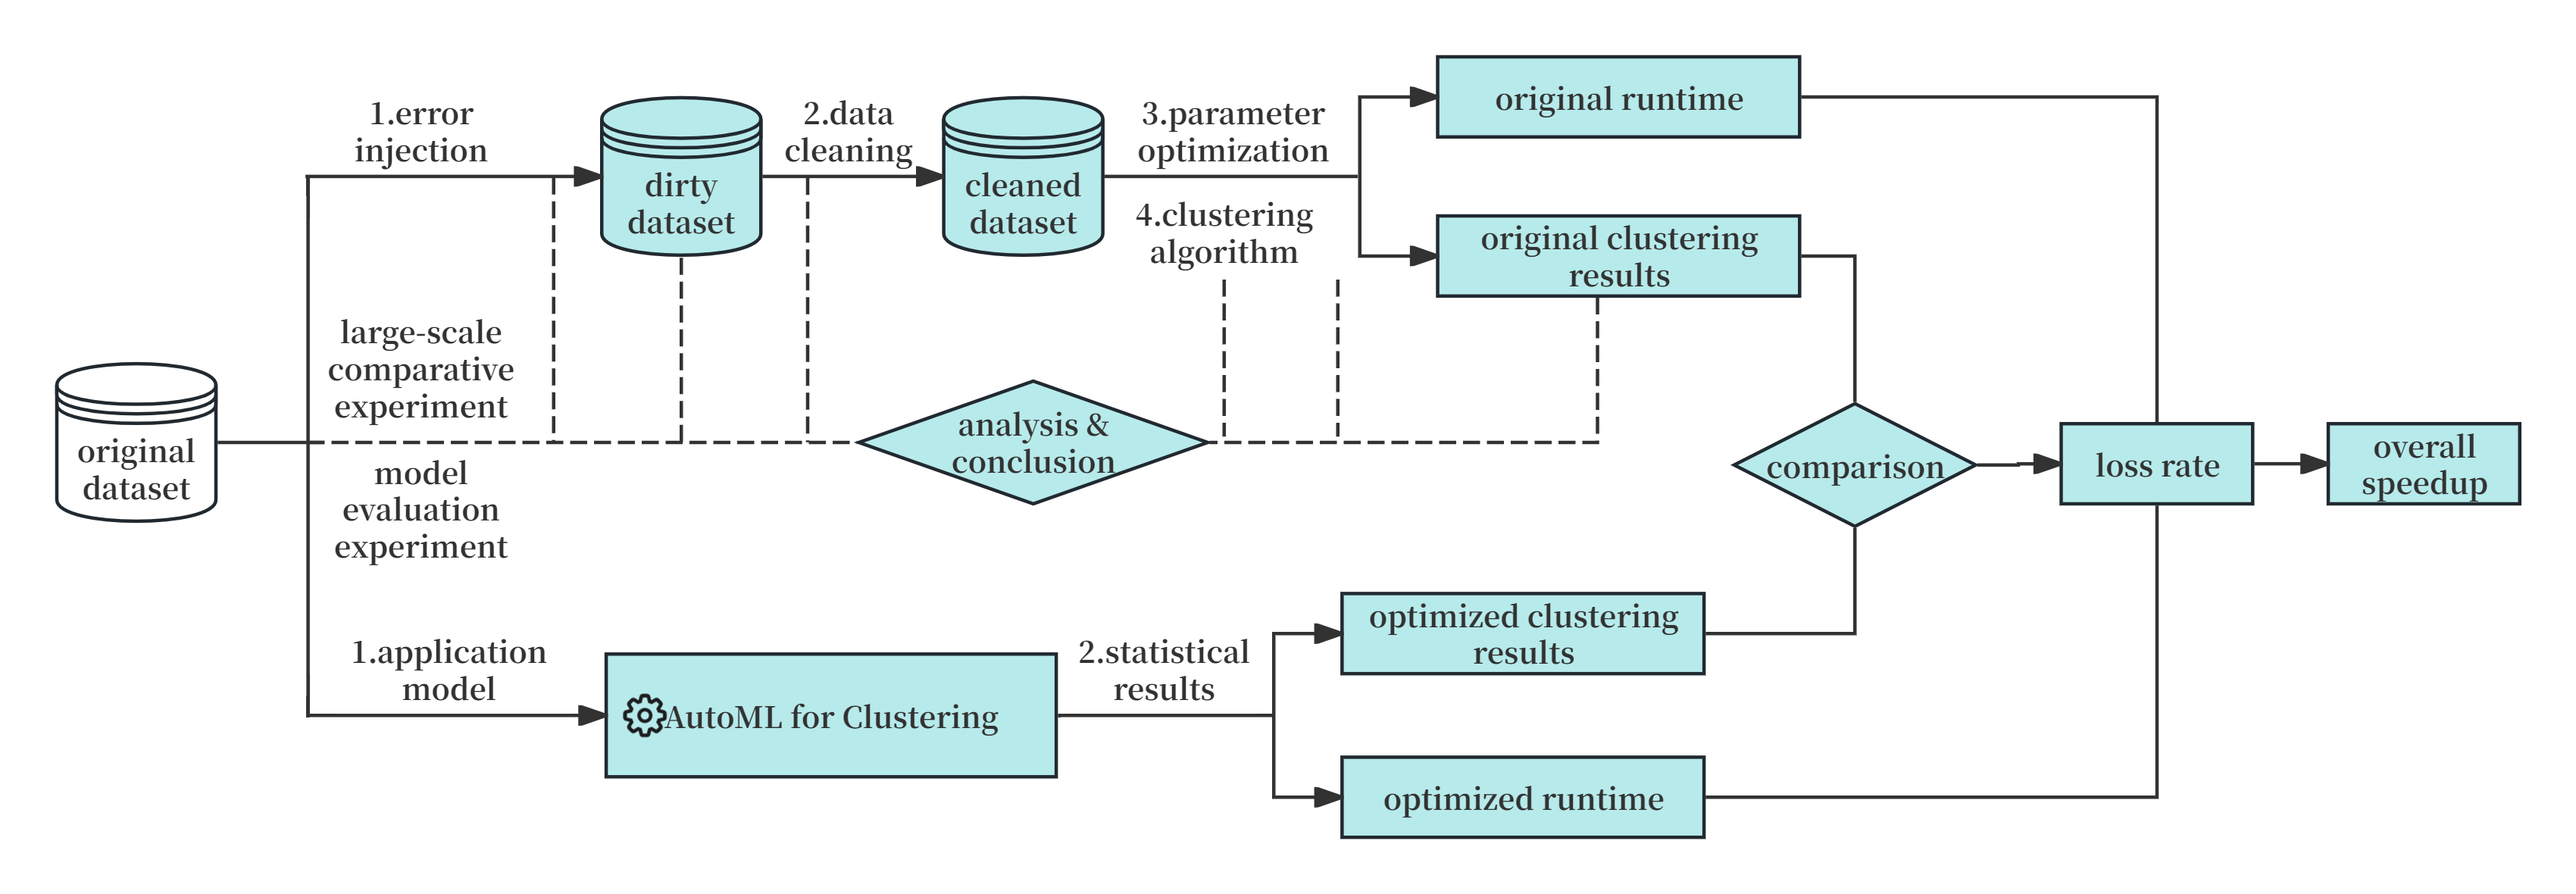
\includegraphics[width=1.0\linewidth]{figures/exp_workflow.png}
    \caption{实验设计流程示意图}
    \label{fig:exp_workflow}
\end{figure}

\begin{enumerate}
    \item \textbf{错误注入与特征统计}:  
    在原始数据集上人为注入不同比例的错误(包括缺失值、噪声和异常值),模拟真实数据质量问题。随后,统计各数据集的错误率、缺失率及噪声水平,提取数据特征向量 \(\mathbf{x}(D)\),为后续清洗与聚类优化提供基础记录。

    \item \textbf{清洗与聚类执行}:  
    依次应用不同的数据清洗策略,对每个数据集生成多个修复版本;随后,在清洗后的数据集上运行各种聚类算法,并记录对应的超参数、聚类簇数、运行时间及综合得分 \(S(D,\omega)\)(计算见式 \eqref{eq:S-score})。

    \item \textbf{结果分析}:  
    比较不同清洗-聚类组合的性能,评估其聚类质量、计算耗时及适用性,分析数据质量对聚类效果的影响,并总结最优策略的适配性。

    \item \textbf{自动化优化}:  
    在离线阶段训练多标签分类器,学习“数据特征 \(\mathbf{x}(D)\) → 优选子空间 \(\Omega'(D)\)”的映射关系;在测试阶段,该模型将用于高效推荐清洗-聚类方案,并与全量搜索结果进行对比,计算损失率 \(\eta(D)\) 和加速比 \(\mathcal{A}(D)\) 。
\end{enumerate}

该流程确保了实验在不同场景下的准确性和可复现性,并为后续实验提供统一框架。

在接下来的部分,我们将围绕两项核心任务展开:
\begin{itemize}
    \item \textbf{大规模对比实验(第~\ref{sec:large_scale_exp} 节)}:  
    评估各种清洗-聚类组合在全部数据集上的表现,分析最优策略在不同数据质量条件下的适配性。

    \item \textbf{自动化聚类模型评估实验(第~\ref{sec:automl_exp} 节)}:  
    验证自动化管线的有效性,对比多标签学习推荐的“优选子空间搜索”与“全量搜索”,重点考察损失率 \(\eta(D)\) 及加速比 \(\mathcal{A}(D)\)两个指标,评估其在大规模数据场景下的可行性。
\end{itemize}

\subsection{大规模对比实验}
\label{sec:large_scale_exp}

本节针对“清洗策略 + 聚类算法”协同优化进行大规模对比实验,以回答第~\ref{subsec:problem-formalization} 节提出的核心问题:
\emph{“不同清洗-聚类组合在多样化数据(含噪声、缺失值、错误值)上的协同表现如何?”}

\subsubsection{实验设置与评估指标}
\label{sec:exp_setting_largeset}

\paragraph{清洗-聚类组合}
对每个数据集分别应用 mode、Raha-Baran 及 GT 三种清洗方法,并运行 K-Means、DBSCAN、OPTICS、HC、GMM 和 AffinityPropagation 六种聚类算法,形成“3 清洗 × 6 聚类 = 18” 种组合。

\paragraph{评估指标}
本研究主要使用以下三个指标来评估清洗-聚类组合的效果:

\begin{itemize}
    \item \textbf{簇数量合理性}:  
    为确保聚类结果的有效性,簇数量应在以下范围内:  
    \begin{itemize}
        \item 标准范围:簇数量通常不小于 5 个,且不大于样本数的算术平方根。
        \item 筛选规则:若簇数明显偏离此范围(例如过少导致过度聚合,或过多导致过度分散),则视为不合法结果并排除。
    \end{itemize}
    
    \item \textbf{综合得分}:  
    综合得分 \(S(D,\omega)\) 的权重设置为 \(\alpha = 0.75\) 和 \(\beta = 0.25\),这一选择基于预实验结果。过高的轮廓系数权重会导致簇数过少,与实际需求不符。因此,较低的 \(\beta\) 权重有助于生成数量合适且更稳定的簇。

    \item \textbf{百分比得分}:  
    为了便于比较不同算法组合之间的性能,本研究对综合得分进行百分比归一化处理,以 GroundTruth 清洗策略修复后的最高综合得分为基准,将其定义为 100\%。不合理的实验结果(如算法运行超时、不收敛或簇数明显偏离标准范围)被标记为 0\%,以避免其干扰整体结果的分析。

\end{itemize}

\subsubsection{实验结果与分析}
\label{sec:exp_result_all}
本节围绕不同数据集上策略组合的性能展开实验结果呈现和分析。我们从以下三个层面展开讨论:
\paragraph{(1) 各数据集在不同错误率下的最优方案与得分情况}  
图~\ref{fig:beers_error}、\ref{fig:flights_error}、\ref{fig:rayyan_error} 和 \ref{fig:hospital_error} 分别展示了 \textit{beers}、\textit{flights}、\textit{rayyan} 与 \textit{hospital} 四个数据集在不同比例错误率(横轴)下的百分比综合得分(左侧纵轴)及缺失值比例(右侧纵轴)。我们引入了\textbf{最接近基准的组合},其得分是除参考标准外距离 100\% 最近的方案。该方案的选取有助于识别在实际应用中最接近理想基准性能的策略。

\begin{figure}[H]
    \centering
    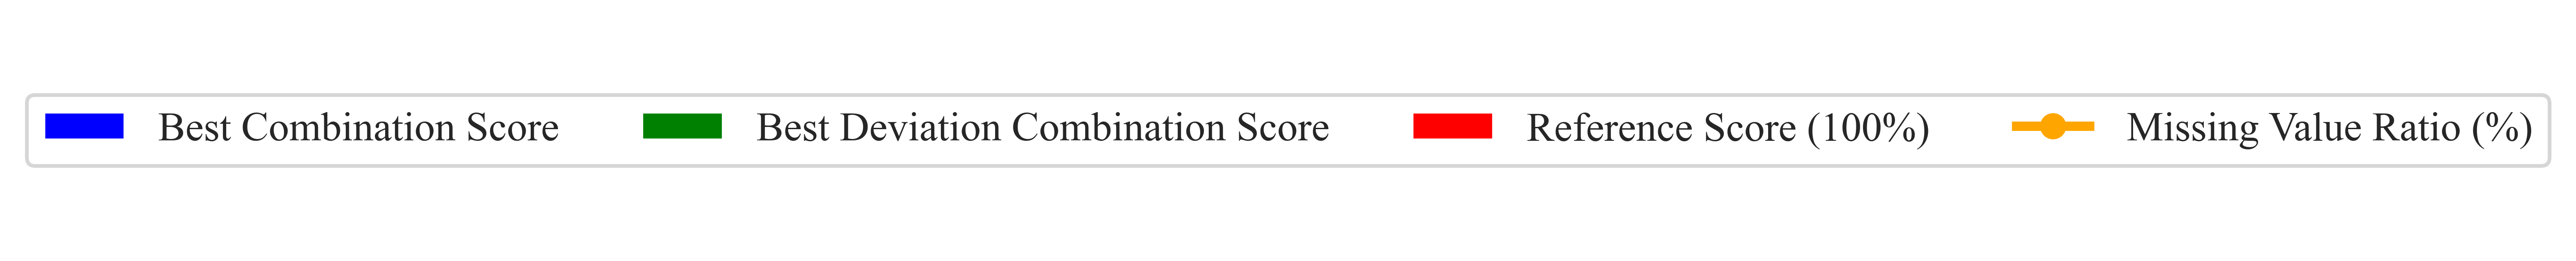
\includegraphics[width=0.9\linewidth]{figures/legend_plot.png} % 确保 legend.png 存在
    \vspace{-14pt} % 减小图例与主图之间的间距
\end{figure}

\begin{figure}[H]
  \centering
  \begin{subfigure}{0.49\linewidth} % 每张图占 48% 宽度
    \centering
    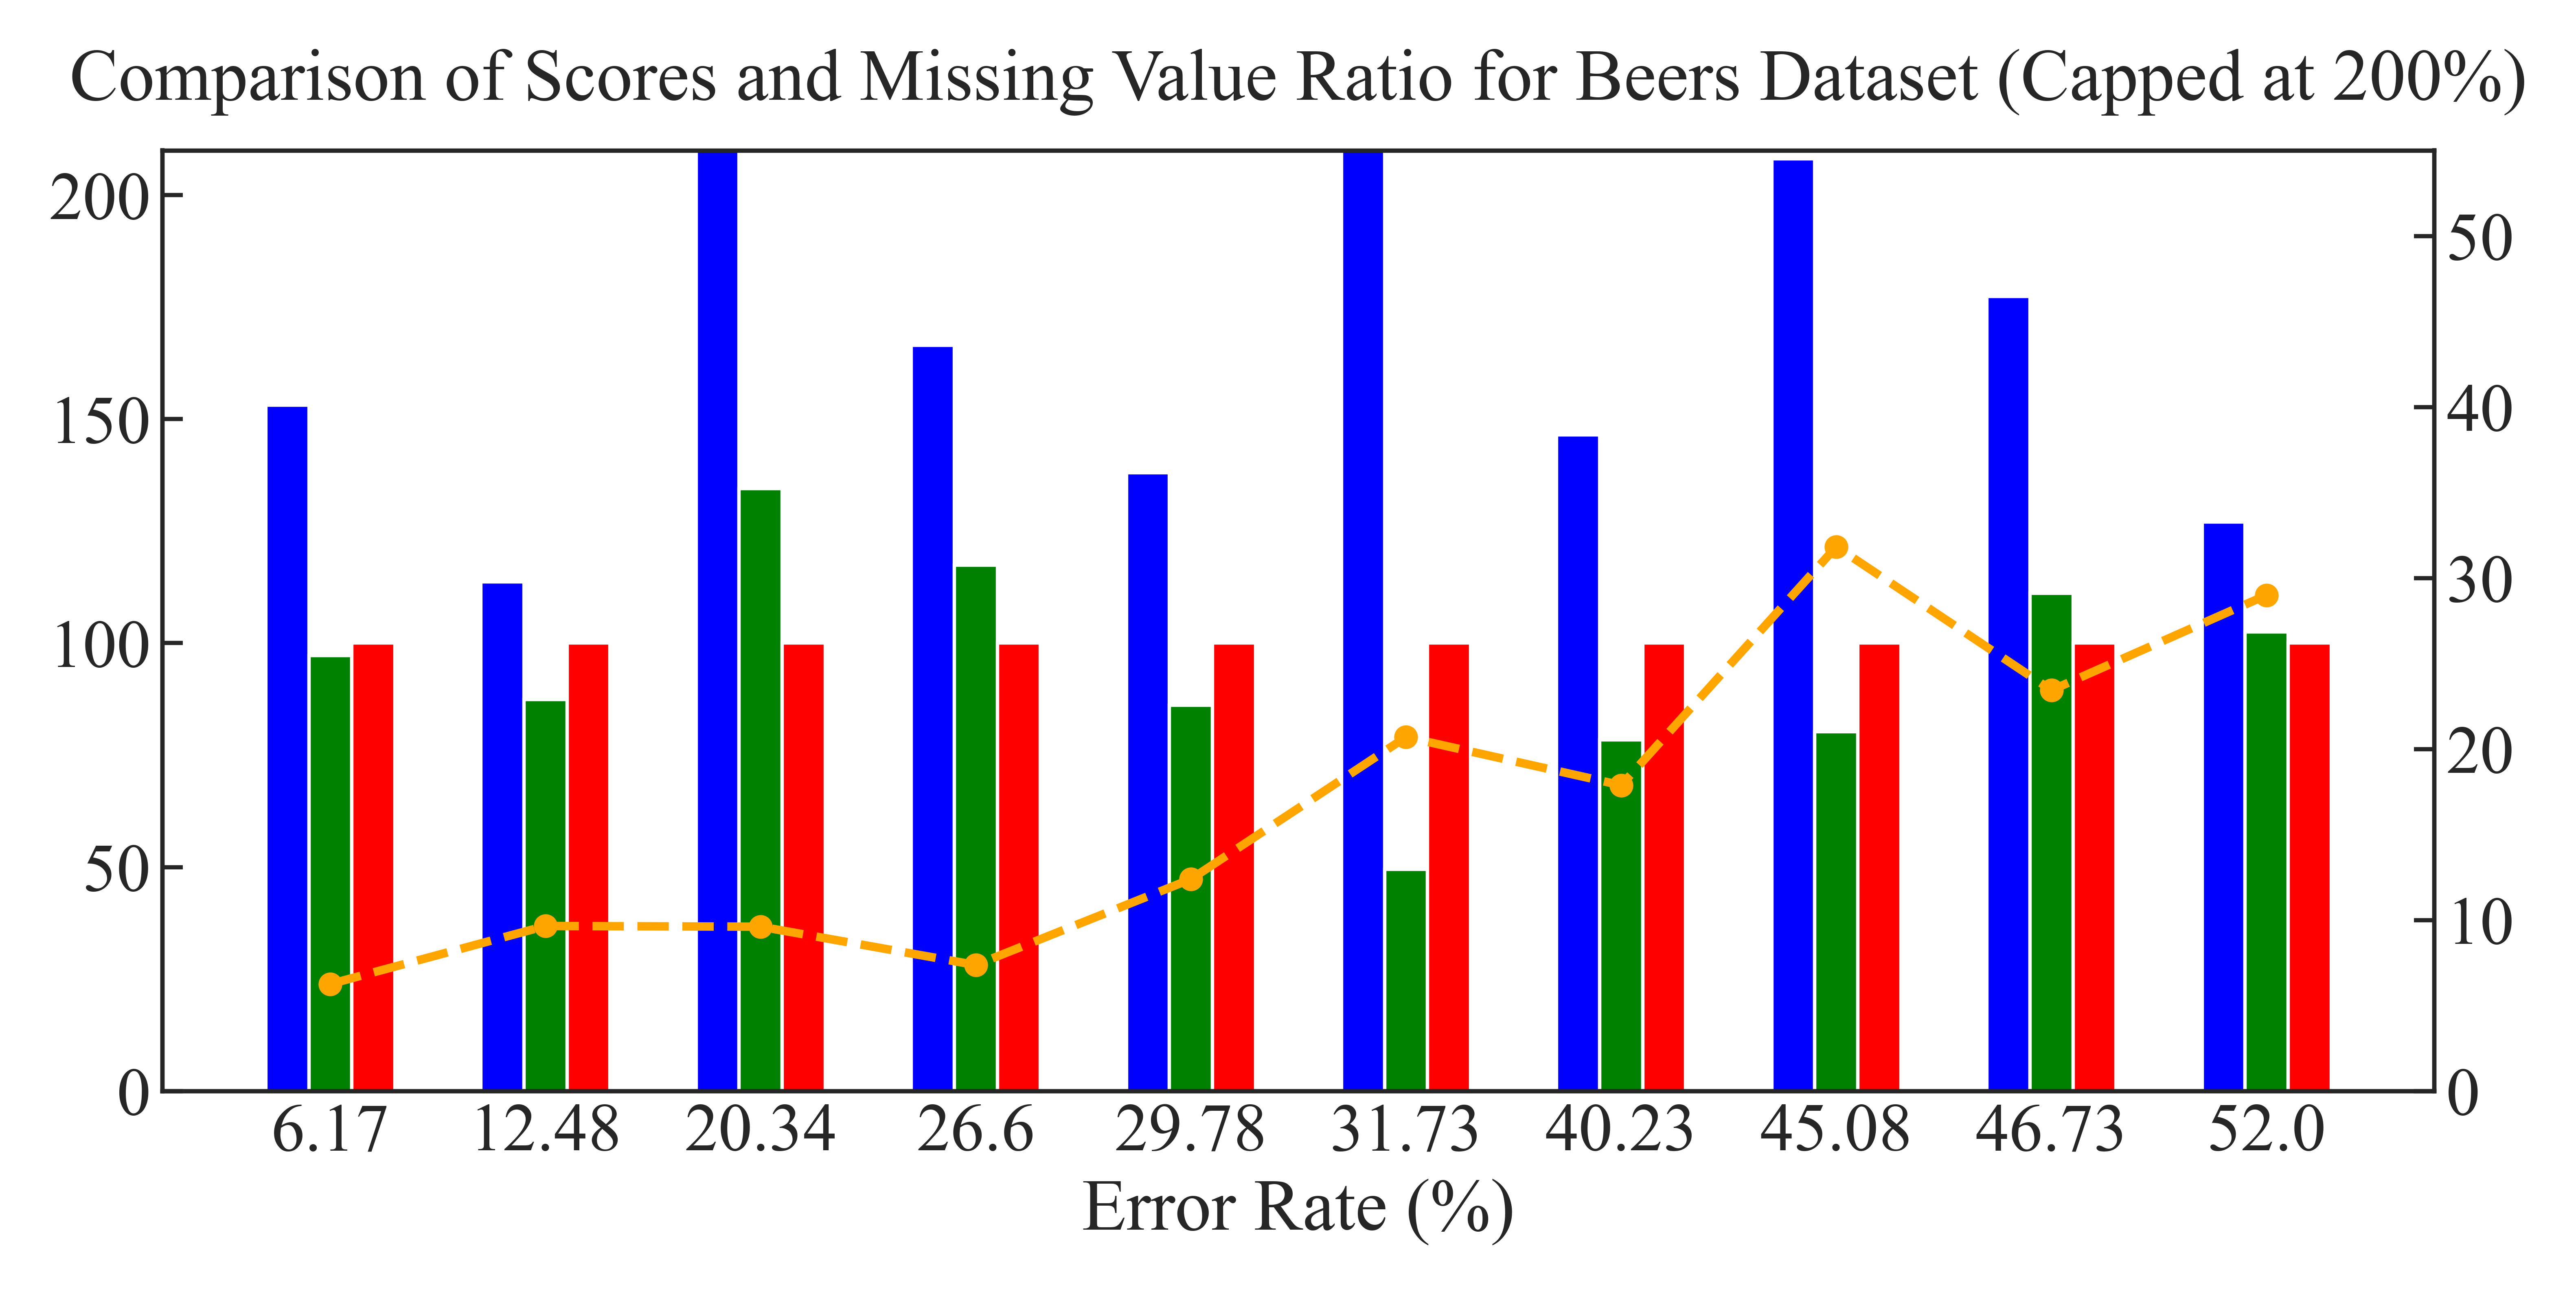
\includegraphics[width=\linewidth]{figures/beers_error.png} % 替换为实际图片
    \caption{\textit{beers} 数据集:错误率 vs. 综合得分与缺失值比例}
    \label{fig:beers_error}
  \end{subfigure}
  \hfill
  \begin{subfigure}{0.49\linewidth}
    \centering
    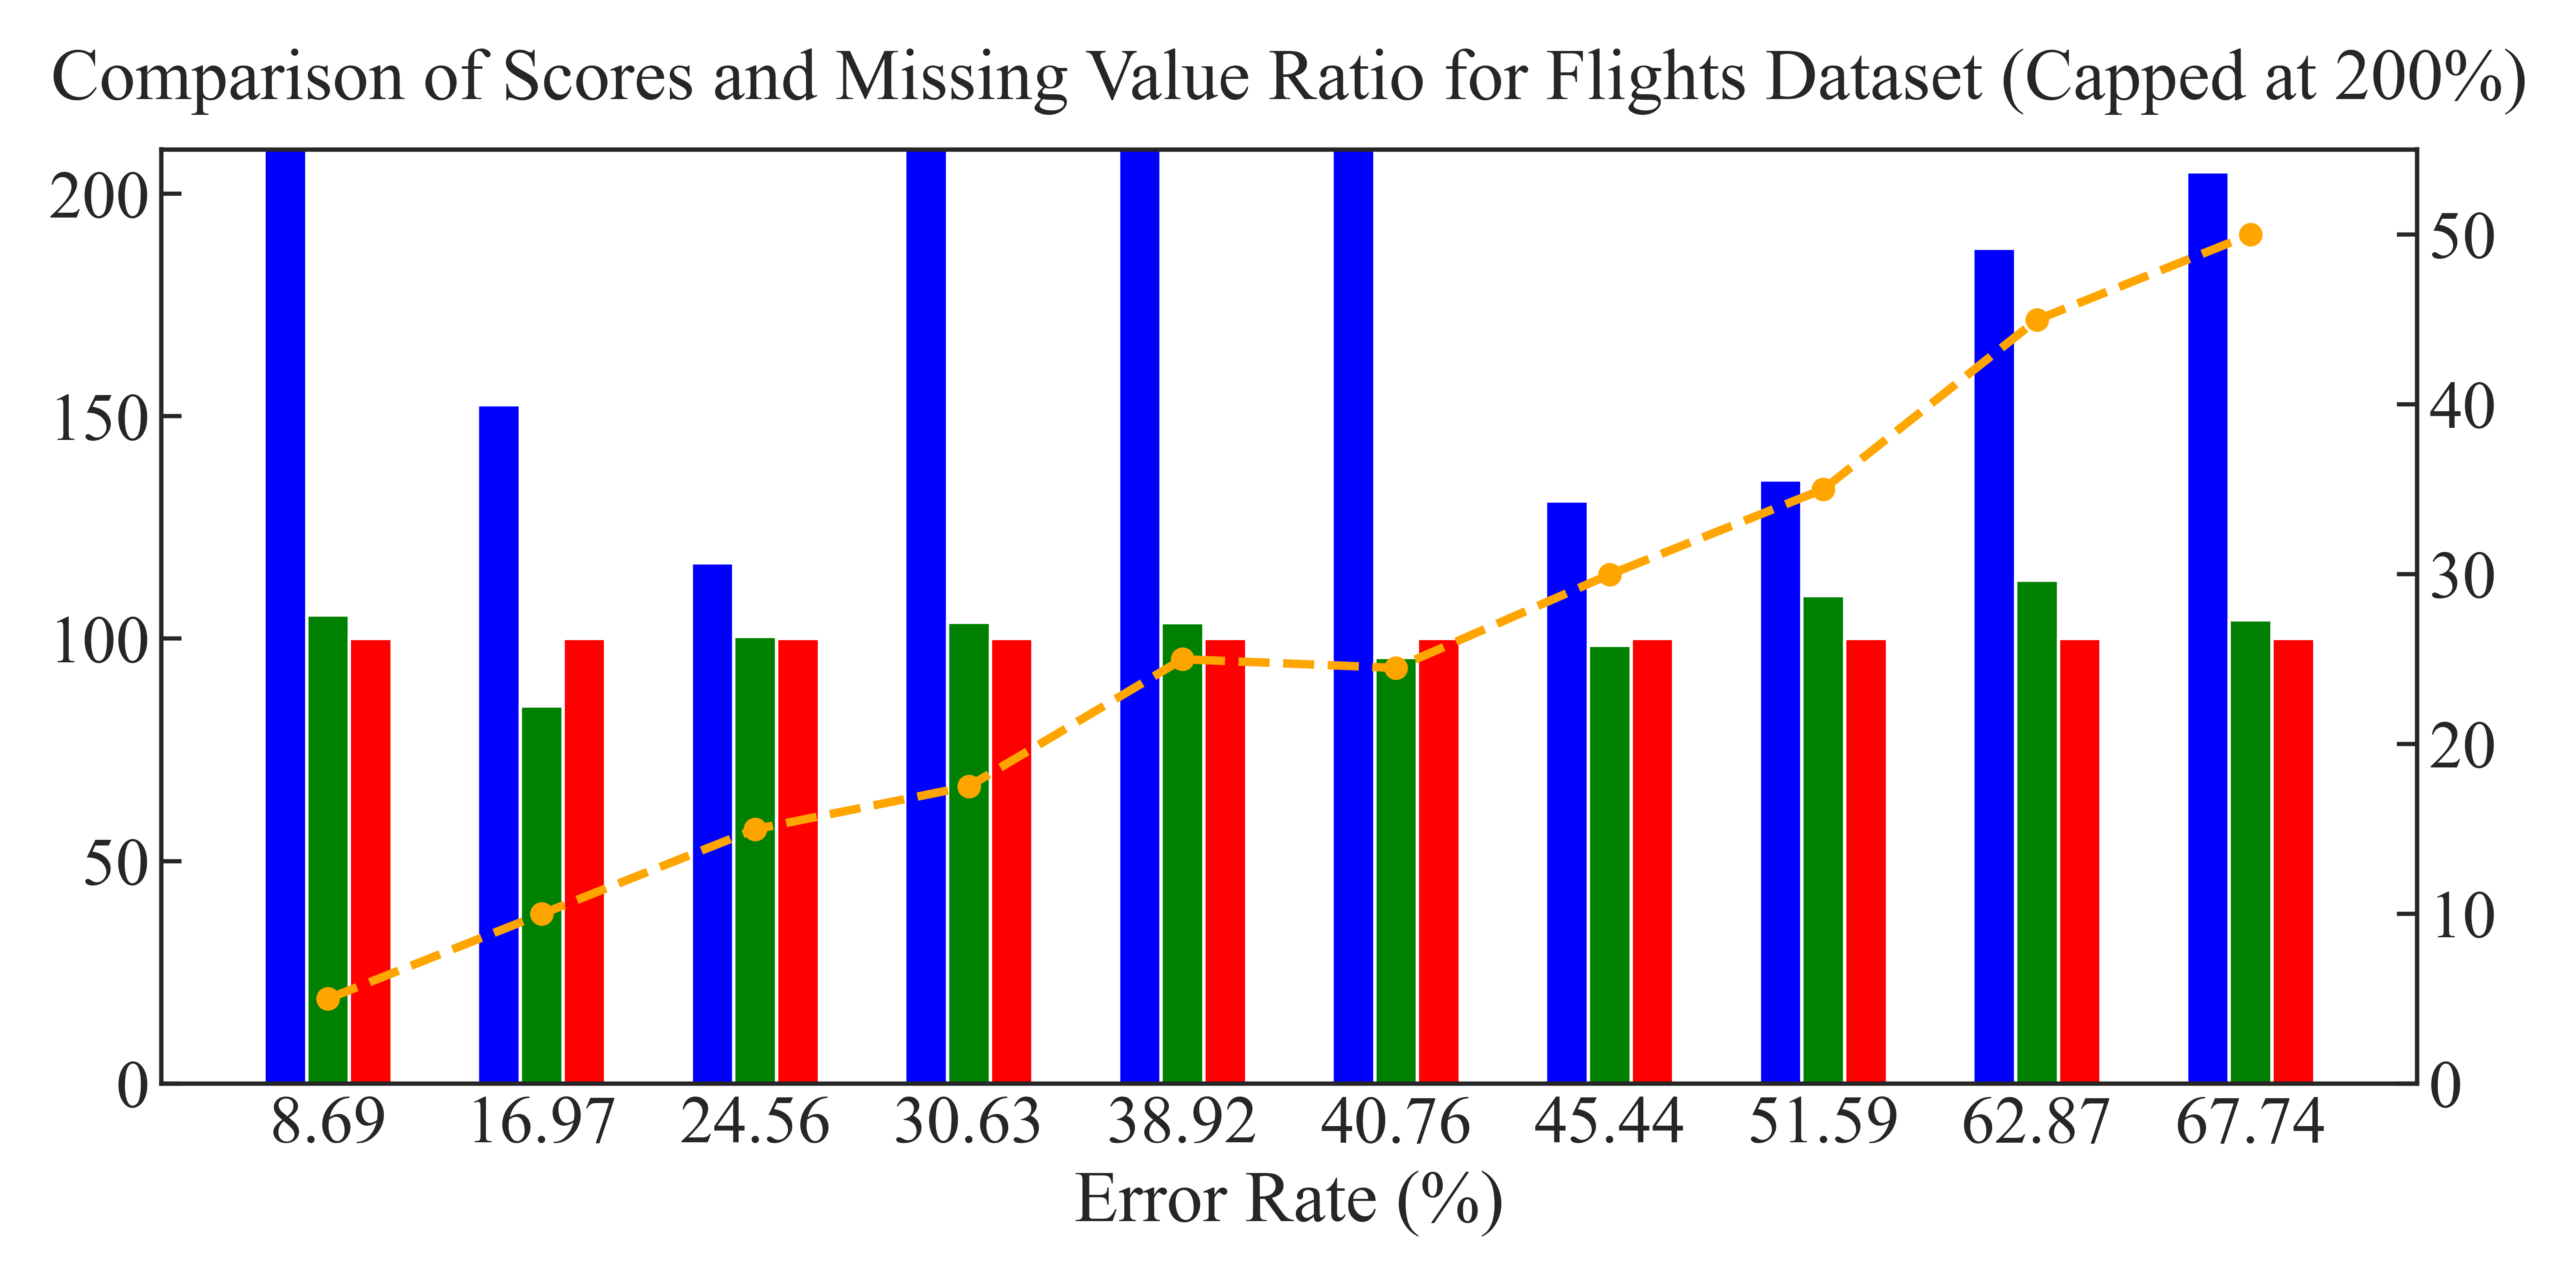
\includegraphics[width=\linewidth]{figures/flights_error.png}
    \caption{\textit{flights} 数据集:错误率 vs. 综合得分与缺失值比例}
    \label{fig:flights_error}
  \end{subfigure}

  \vspace{0.5em} % 调整行间距

  \begin{subfigure}{0.49\linewidth}
    \centering
    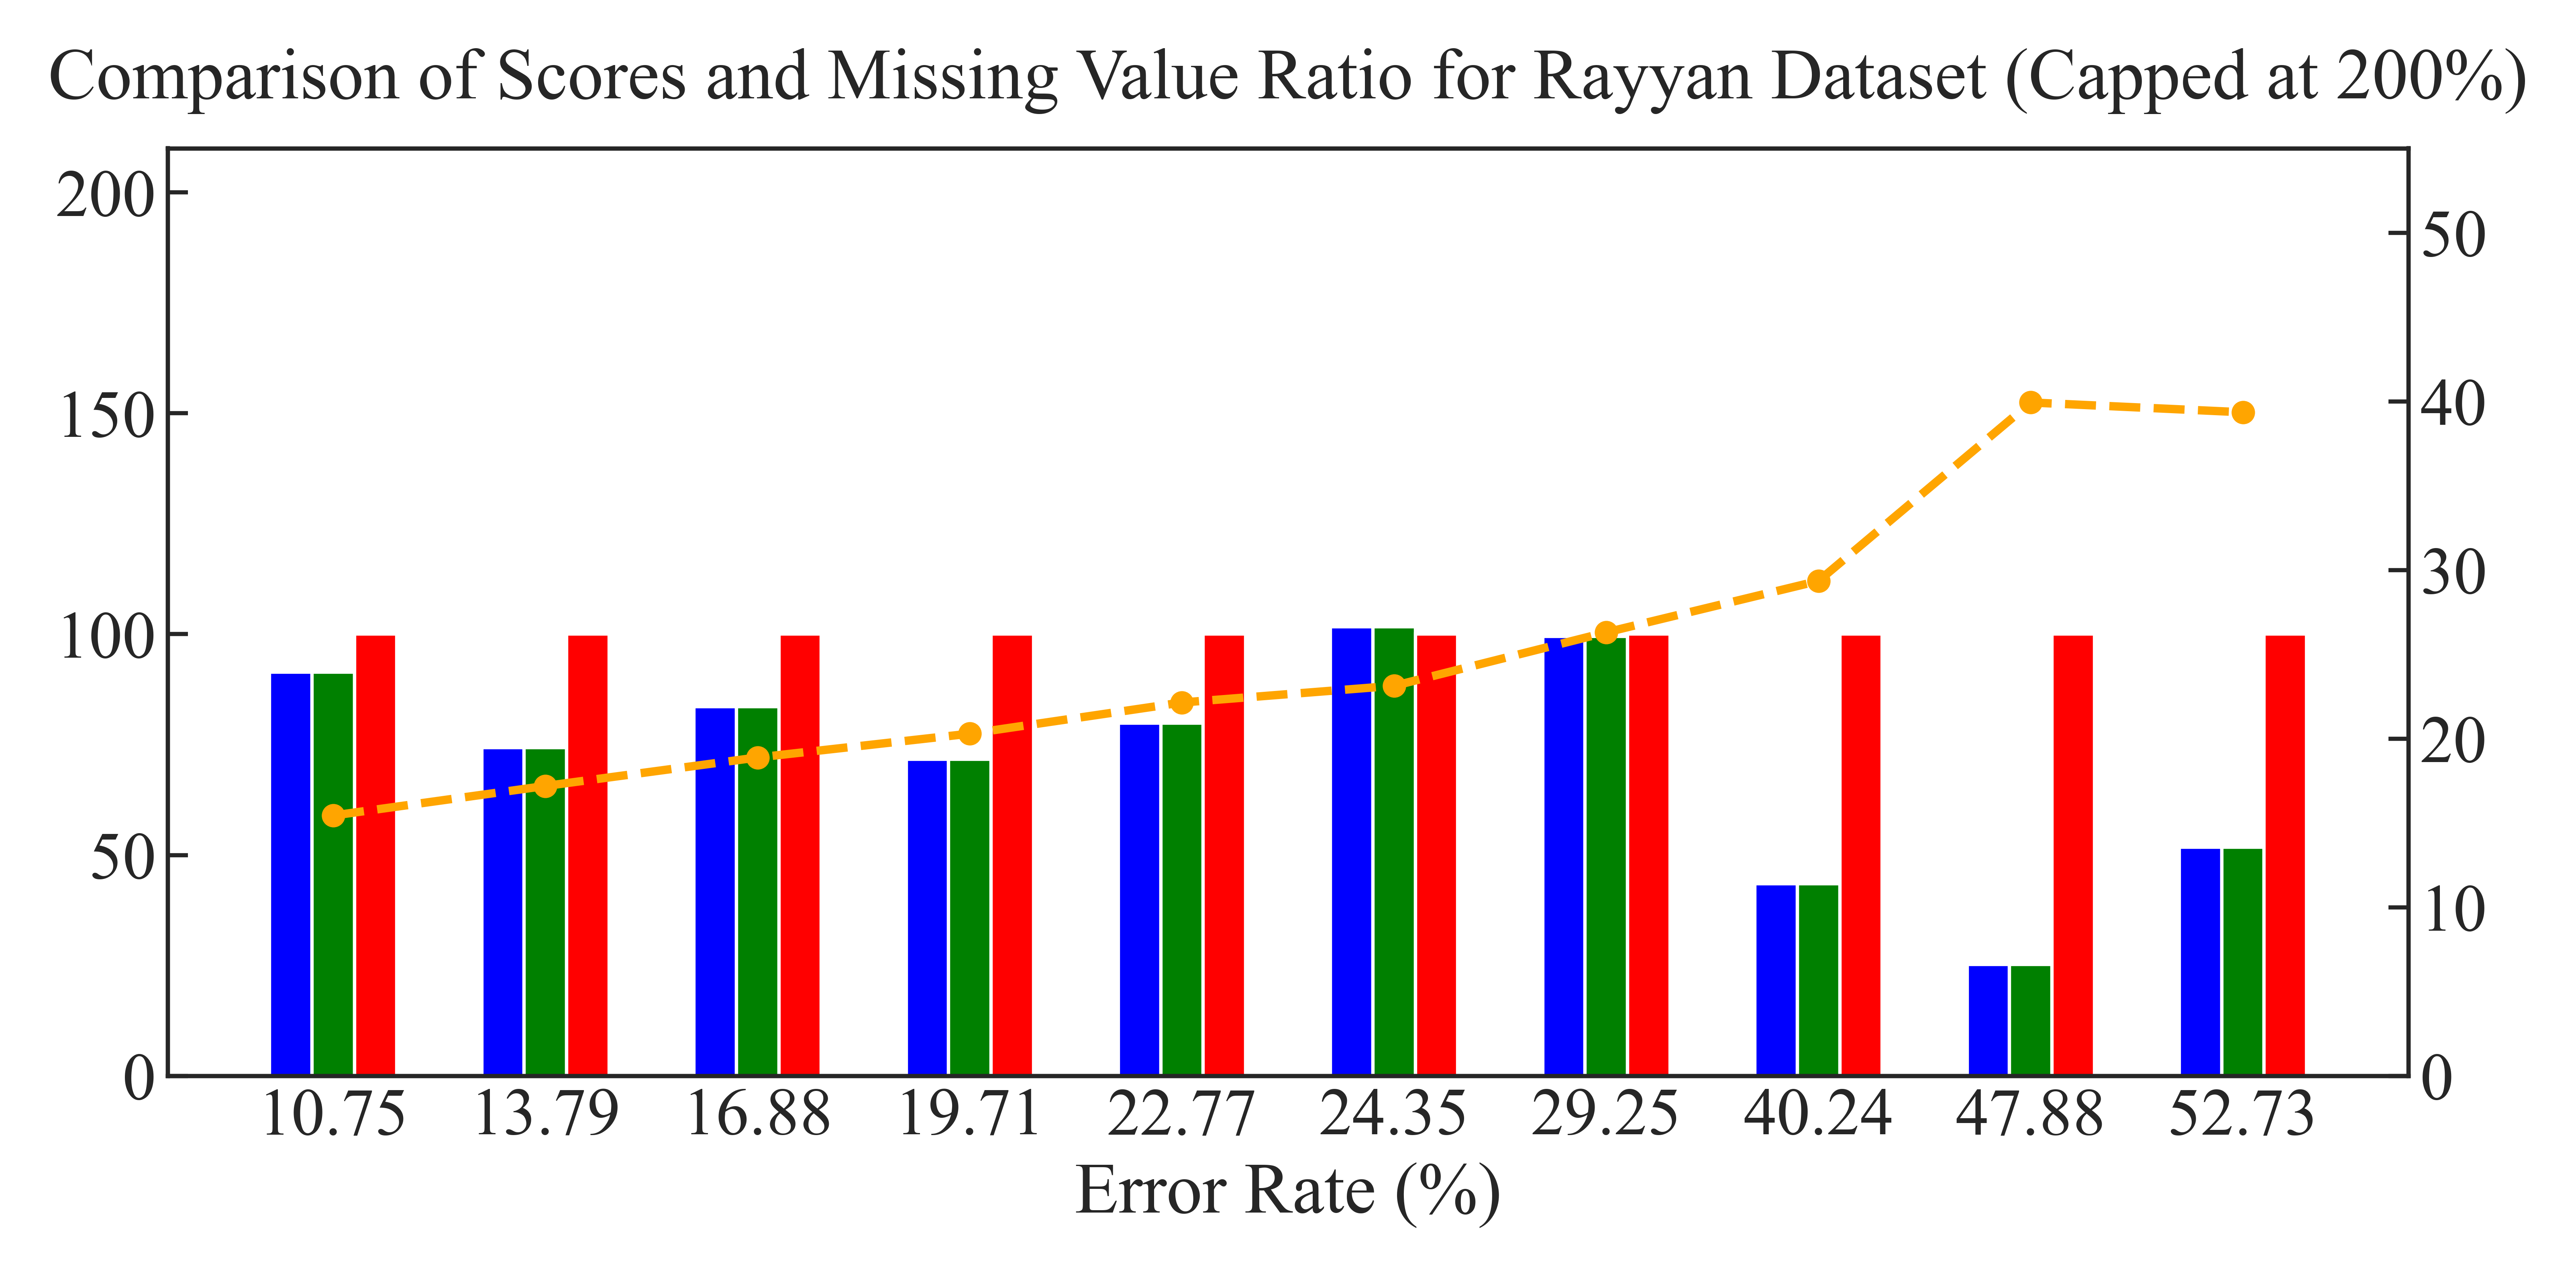
\includegraphics[width=\linewidth]{figures/rayyan_error.png}
    \caption{\textit{rayyan} 数据集:错误率 vs. 综合得分与缺失值比例}
    \label{fig:rayyan_error}
  \end{subfigure}
  \hfill
  \begin{subfigure}{0.49\linewidth}
    \centering
    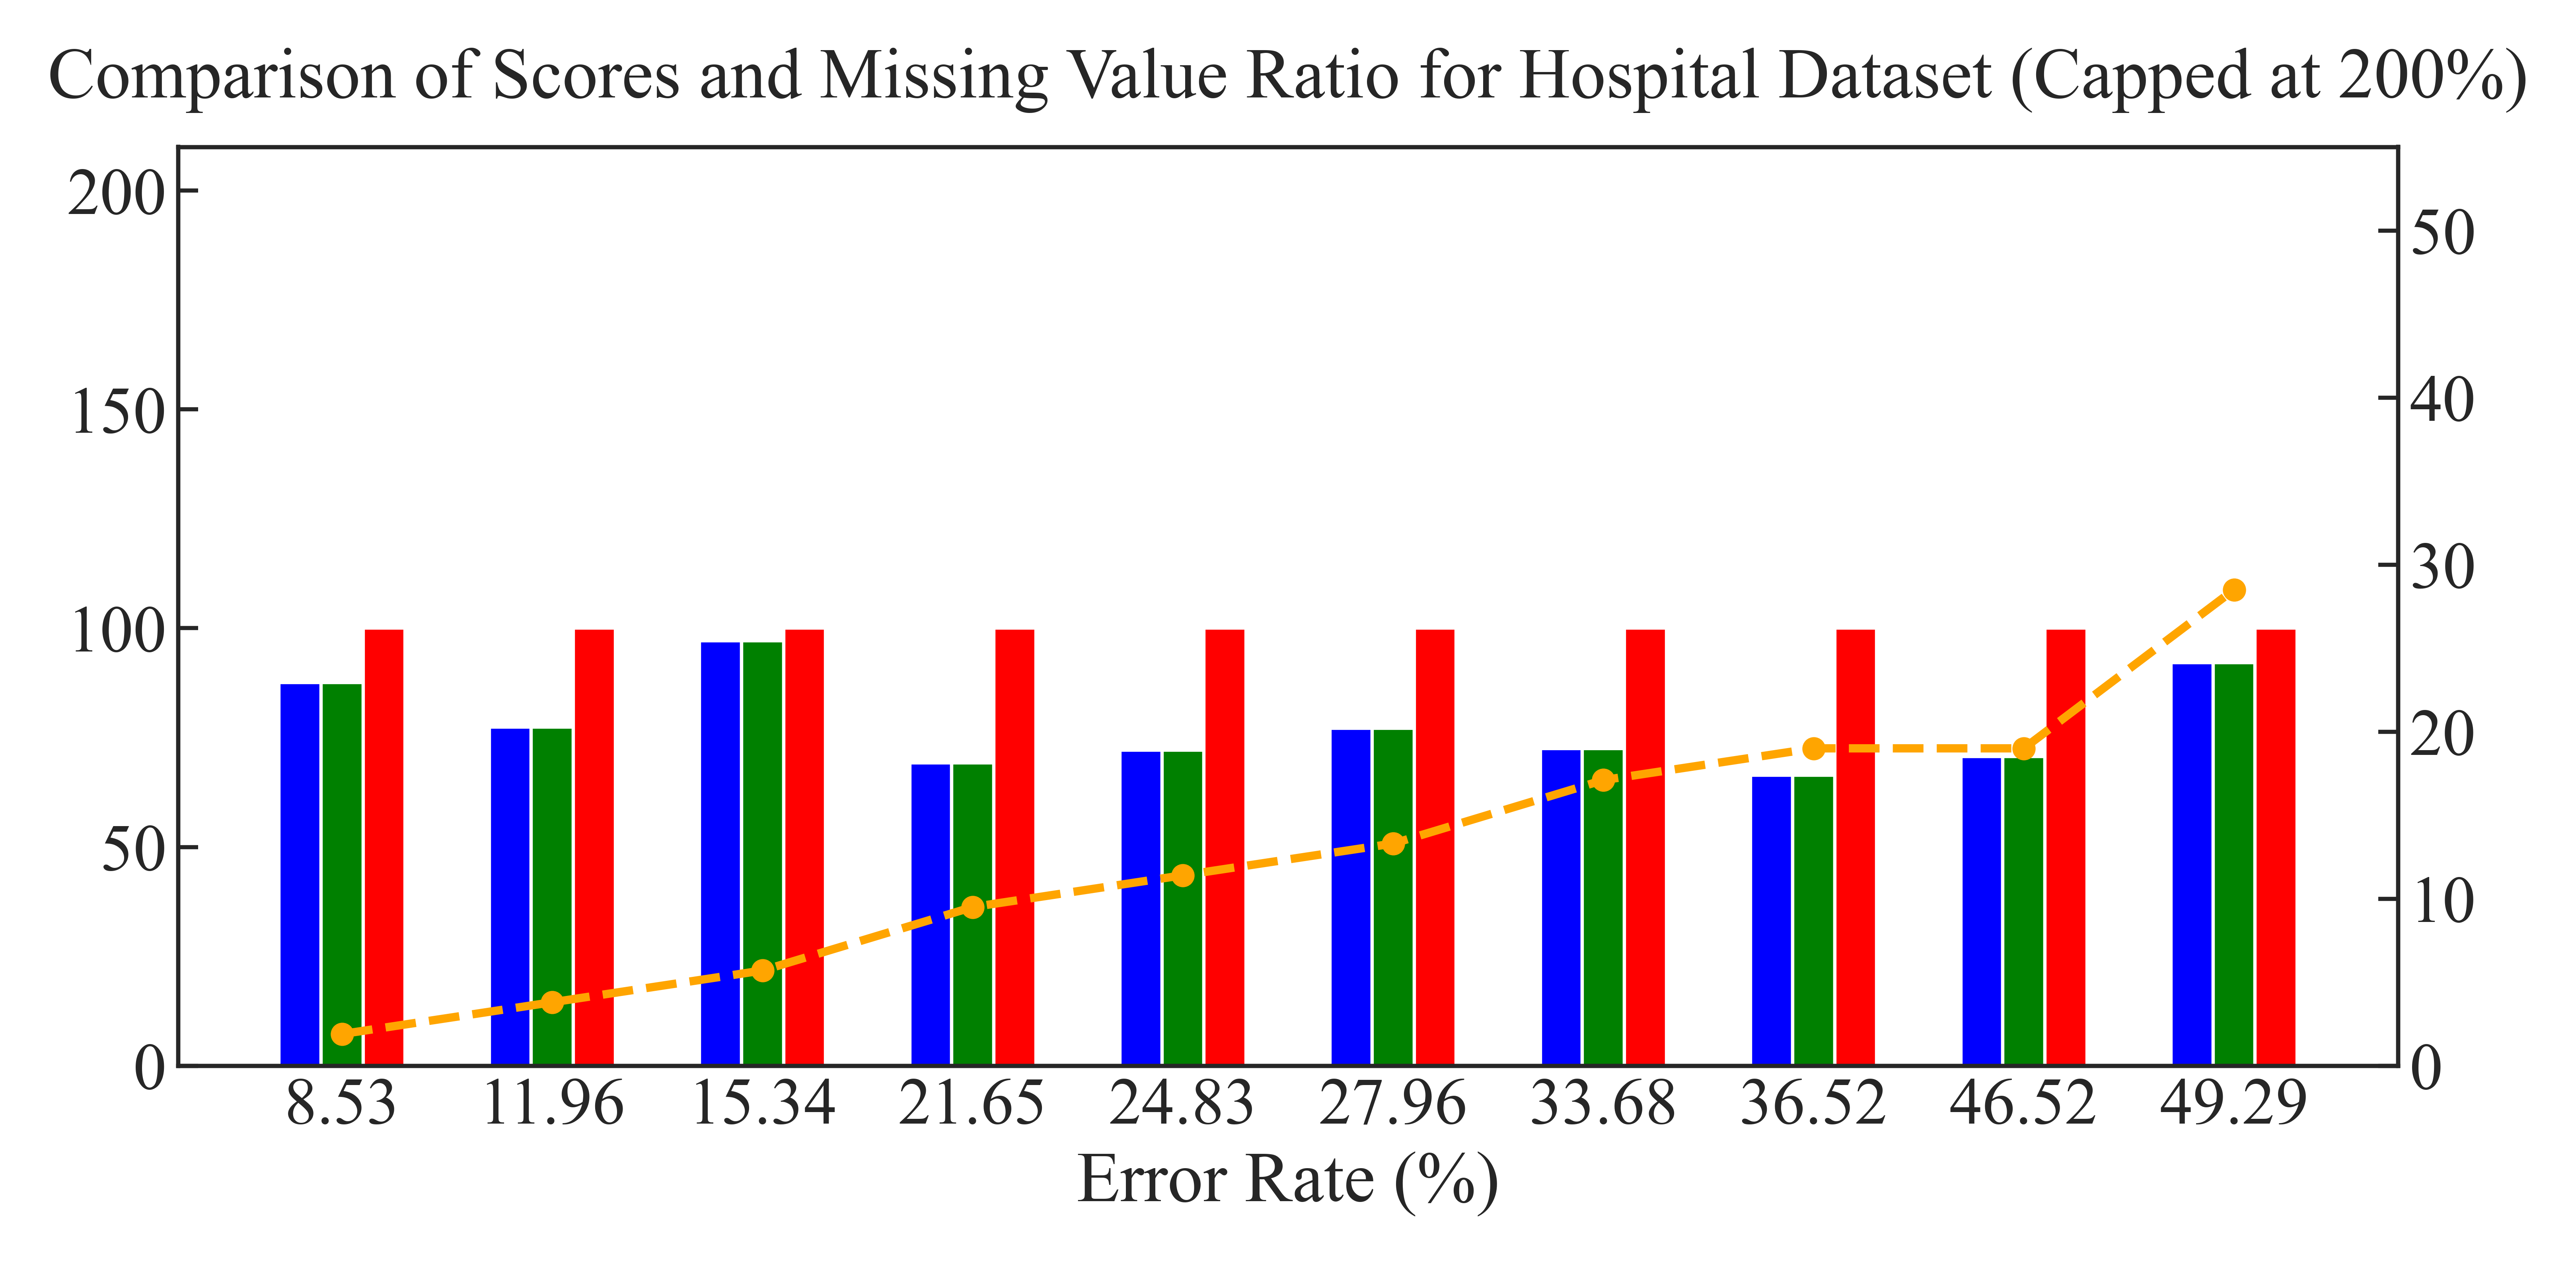
\includegraphics[width=\linewidth]{figures/hospital_error.png}
    \caption{\textit{hospital} 数据集:错误率 vs. 综合得分与缺失值比例}
    \label{fig:hospital_error}
  \end{subfigure}

  \caption{不同数据集在不同错误率条件下的得分与缺失值比例变化}
  \label{fig:all_datasets}
\end{figure}

\vspace{0.5em}
\noindent
通过以上四张图可以观察到,随着错误率的增加,各数据集的缺失值比例呈现不同程度的波动。此外,不同清洗-聚类组合在部分数据条件下表现出显著差异,其中某些方案的得分甚至远超基准值(超过 200\%)。为了更详细地分析这些现象,表~\ref{tab:beers_results} 至~\ref{tab:hospital_results} 进一步列出了四个数据集在不同错误率下的\textbf{最佳方案}(\textit{Best Combination}, C$_1$) 及其综合得分 (\textit{Best Score}, S$_1$),同时给出了\textbf{最接近基准的组合}(\textit{Best Deviation Combination}, C$_2$) 及其对应得分 (\textit{Best Deviation Score}, S$_2$)。这些结果有助于我们深入理解不同清洗-聚类组合的适用性,并评估其对聚类质量的影响。

\begin{table}[htbp]
    \centering
    \footnotesize % 适中字体
    \setlength{\tabcolsep}{4pt} % 调整列间距
    \renewcommand{\arraystretch}{1.1} % 增加行距,提高可读性
    \begin{subtable}{0.48\linewidth} % beers 数据集
        \centering
        \caption{\textit{beers} 数据集}
        \label{tab:beers_results}
        \begin{tabular}{lccccc}
            \toprule
            \textbf{Name} & \textbf{Error (\%)} & \textbf{C$_1$} & \textbf{S$_1$ (\%)} & \textbf{C$_2$} & \textbf{S$_2$ (\%)} \\
            \midrule
            beers & 6.17  & mode + HC  & 153.11 & R-B + HC  & 97.21 \\
            beers & 12.48 & R-B + HC   & 113.69 & mode + HC & 87.37 \\
            beers & 20.34 & mode + HC  & 259.85 & R-B + HC  & 134.50 \\
            beers & 26.60 & mode + HC  & 166.54 & mode + AP & 117.45 \\
            beers & 29.78 & R-B + HC   & 138.07 & mode + HC & 86.14 \\
            beers & 31.73 & mode + AP  & 232.95 & mode + DB & 49.49 \\
            beers & 40.23 & mode + HC  & 146.54 & mode + KM & 78.38 \\
            beers & 45.08 & mode + HC  & 208.15 & R-B + HC  & 80.19 \\
            beers & 46.73 & mode + HC  & 177.37 & mode + AP & 111.11 \\
            beers & 52.00 & mode + HC  & 127.06 & mode + DB & 102.51 \\
            \bottomrule
        \end{tabular}
    \end{subtable}
    \hfill
    \begin{subtable}{0.48\linewidth} % flights 数据集
        \centering
        \caption{\textit{flights} 数据集}
        \label{tab:flights_results}
        \begin{tabular}{lccccc}
            \toprule
            \textbf{Name} & \textbf{Error (\%)} & \textbf{C$_1$} & \textbf{S$_1$ (\%)} & \textbf{C$_2$} & \textbf{S$_2$ (\%)} \\
            \midrule
            flights & 8.69  & mode + HC  & 290.44 & mode + KM  & 105.36 \\
            flights & 16.97 & mode + GMM & 152.61 & R-B + HC   & 84.89 \\
            flights & 24.56 & R-B + HC   & 117.03 & R-B + AP   & 100.53 \\
            flights & 30.63 & mode + DB  & 242.21 & mode + GMM & 103.68 \\
            flights & 38.92 & mode + DB  & 1817.80 & mode + GMM & 103.55 \\
            flights & 40.76 & mode + DB  & 2543.51 & mode + AP  & 95.80 \\
            flights & 45.44 & mode + AP  & 130.95 & mode + DB  & 98.48 \\
            flights & 51.59 & mode + HC  & 135.66 & R-B + HC   & 109.68 \\
            flights & 62.87 & mode + KM  & 187.77 & R-B + HC   & 113.10 \\
            flights & 67.74 & mode + HC  & 204.94 & R-B + HC   & 104.27 \\
            \bottomrule
        \end{tabular}
    \end{subtable}

    \vspace{0.5em} % 适当增加表格间的垂直间距

    \begin{subtable}{0.48\linewidth} % rayyan 数据集
        \centering
        \caption{\textit{rayyan} 数据集}
        \label{tab:rayyan_results}
        \begin{tabular}{lccccc}
            \toprule
            \textbf{Name} & \textbf{Error (\%)} & \textbf{C$_1$} & \textbf{S$_1$ (\%)} & \textbf{C$_2$} & \textbf{S$_2$ (\%)} \\
            \midrule
            rayyan & 10.75  & R-B + HC  & 91.38  & R-B + HC  & 91.38  \\
            rayyan & 13.79  & R-B + HC  & 74.35  & R-B + HC  & 74.35  \\
            rayyan & 16.88  & R-B + HC  & 83.63  & R-B + HC  & 83.63  \\
            rayyan & 19.71  & mode + HC & 71.69  & mode + HC & 71.69  \\
            rayyan & 22.77  & R-B + HC  & 79.87  & R-B + HC  & 79.87  \\
            rayyan & 24.35  & R-B + HC  & 101.71 & R-B + HC  & 101.71 \\
            rayyan & 29.25  & R-B + AP  & 99.49  & R-B + AP  & 99.49  \\
            rayyan & 40.24  & R-B + HC  & 43.52  & R-B + HC  & 43.52  \\
            rayyan & 47.88  & mode + HC & 25.22  & mode + HC & 25.22  \\
            rayyan & 52.73  & mode + HC & 51.75  & mode + HC & 51.75  \\
            \bottomrule
        \end{tabular}
    \end{subtable}
    \hfill
    \begin{subtable}{0.48\linewidth} % hospital 数据集
        \centering
        \caption{\textit{hospital} 数据集}
        \label{tab:hospital_results}
        \begin{tabular}{lccccc}
            \toprule
            \textbf{Name} & \textbf{Error (\%)} & \textbf{C$_1$} & \textbf{S$_1$ (\%)} & \textbf{C$_2$} & \textbf{S$_2$ (\%)} \\
            \midrule
            hospital & 8.53  & R-B + HC  & 87.63  & R-B + HC  & 87.63  \\
            hospital & 11.96 & R-B + HC  & 77.42  & R-B + HC  & 77.42  \\
            hospital & 15.34 & R-B + HC  & 97.14  & R-B + HC  & 97.14  \\
            hospital & 21.65 & R-B + HC  & 69.24  & R-B + HC  & 69.24  \\
            hospital & 24.83 & R-B + HC  & 72.12  & R-B + HC  & 72.12  \\
            hospital & 27.96 & R-B + HC  & 77.16  & R-B + HC  & 77.16  \\
            hospital & 33.68 & R-B + HC  & 72.50  & R-B + HC  & 72.50  \\
            hospital & 36.52 & mode + AP & 66.43  & mode + AP & 66.43  \\
            hospital & 46.52 & mode + HC & 70.70  & mode + HC & 70.70  \\
            hospital & 49.29 & mode + AP & 92.17  & mode + AP & 92.17  \\
            \bottomrule
        \end{tabular}
    \end{subtable}

    \caption{不同错误率下各数据集的最佳组合 (C$_1$) 与最接近基准组合 (C$_2$) 及得分}
    \label{tab:all_results}
\end{table}

\vspace{0.5em}
\noindent
基于图~\ref{fig:beers_error} 至图\ref{fig:hospital_error} 和表~\ref{tab:beers_results} 至表~\ref{tab:hospital_results} 所示的不同错误率下的组合排名与偏差情况,我们可以得出以下几点认识:

\begin{enumerate}
    \item \textbf{“最佳组合”与“最接近基准”经常不一致}\\
    在 \textit{Beers}、\textit{Flights} 等较大规模、数值型为主的数据中,mode + HC 或 mode + DBSCAN 有时会出现 200\%~300\%、甚至逾千的“爆分”情形。然而,这些高分结果往往偏离基准结构较远,原因是 DBSCAN 对噪声/缺失值极度敏感,以及 HC 采用的簇数与理想情况差异较大。此时,Raha-Baran + HC 或 mode + KMeans 虽绝对分值较低,却更贴近 GroundTruth 基准。

    \item \textbf{极端高分分布并不均衡,受数据维度与语义约束影响}\\
    在低维数值型的 \textit{Flights} 数据中,mode + DBSCAN 出现 1800\%~2500\% 极端情况,表明密度聚类对填补策略和超参数高度敏感。而在更高维或包含语义规则的 \textit{Hospital}、\textit{Rayyan} 中,聚类分数通常较温和,极少越过 200\%,暗示 Raha-Baran 修复在此类场景下更能保留合理的分布结构,降低了极端划分的可能。

    \item \textbf{Raha-Baran + HC 在中低错误率下尤为稳健}\\
    在 \textit{Hospital}、\textit{Rayyan} 等数据集中,当错误率低于 25\% 时,Raha-Baran + HC 常同时取得“最高分”与“最贴近基准”的好结果。对于高维、具备一定语义约束且规模中等的场景而言,Raha-Baran 能有效减少噪声干扰,HC 则在数据质量良好时更易逼近基准结构。即使错误率升至 40\% 以上,Raha-Baran + HC 也仅出现有限波动,在高维场景下仍优于其他组合。
\end{enumerate}

\paragraph{(2) 不同数据集上清洗-聚类方案随错误率变化的趋势}
前文表格展示了各数据集在不同错误率下的最佳组合及其与基准的偏差,但仅反映离散的关键数值。为直观观察清洗-聚类组合随错误率变化的趋势,本节通过图~\ref{fig:mode_beers} 至图\ref{fig:raha_baran_hospital} 展示各数据集在两种清洗方法下,不同聚类算法的综合得分变化。横轴为错误率,纵轴为综合得分,各曲线对应不同聚类算法,体现其在不同数据质量条件下的波动情况。
\begin{figure}[H]
    \centering
    
\includegraphics[width=0.6\linewidth]{figures/legend.png} % 确保 legend.png 存在
    \vspace{-10pt} % 减小图例与主图之间的间距
\end{figure}

\begin{figure}[H]
  \centering
  \footnotesize % 控制整体字体大小(子图内文本)
  \setlength{\abovecaptionskip}{2pt} % 调整标题和图片之间的间距
  \setlength{\belowcaptionskip}{0pt} % 让 caption 和正文的间距更小

  % 第一行:mode 清洗
  \begin{subfigure}{0.48\linewidth} % 图片尺寸增大
    \centering
    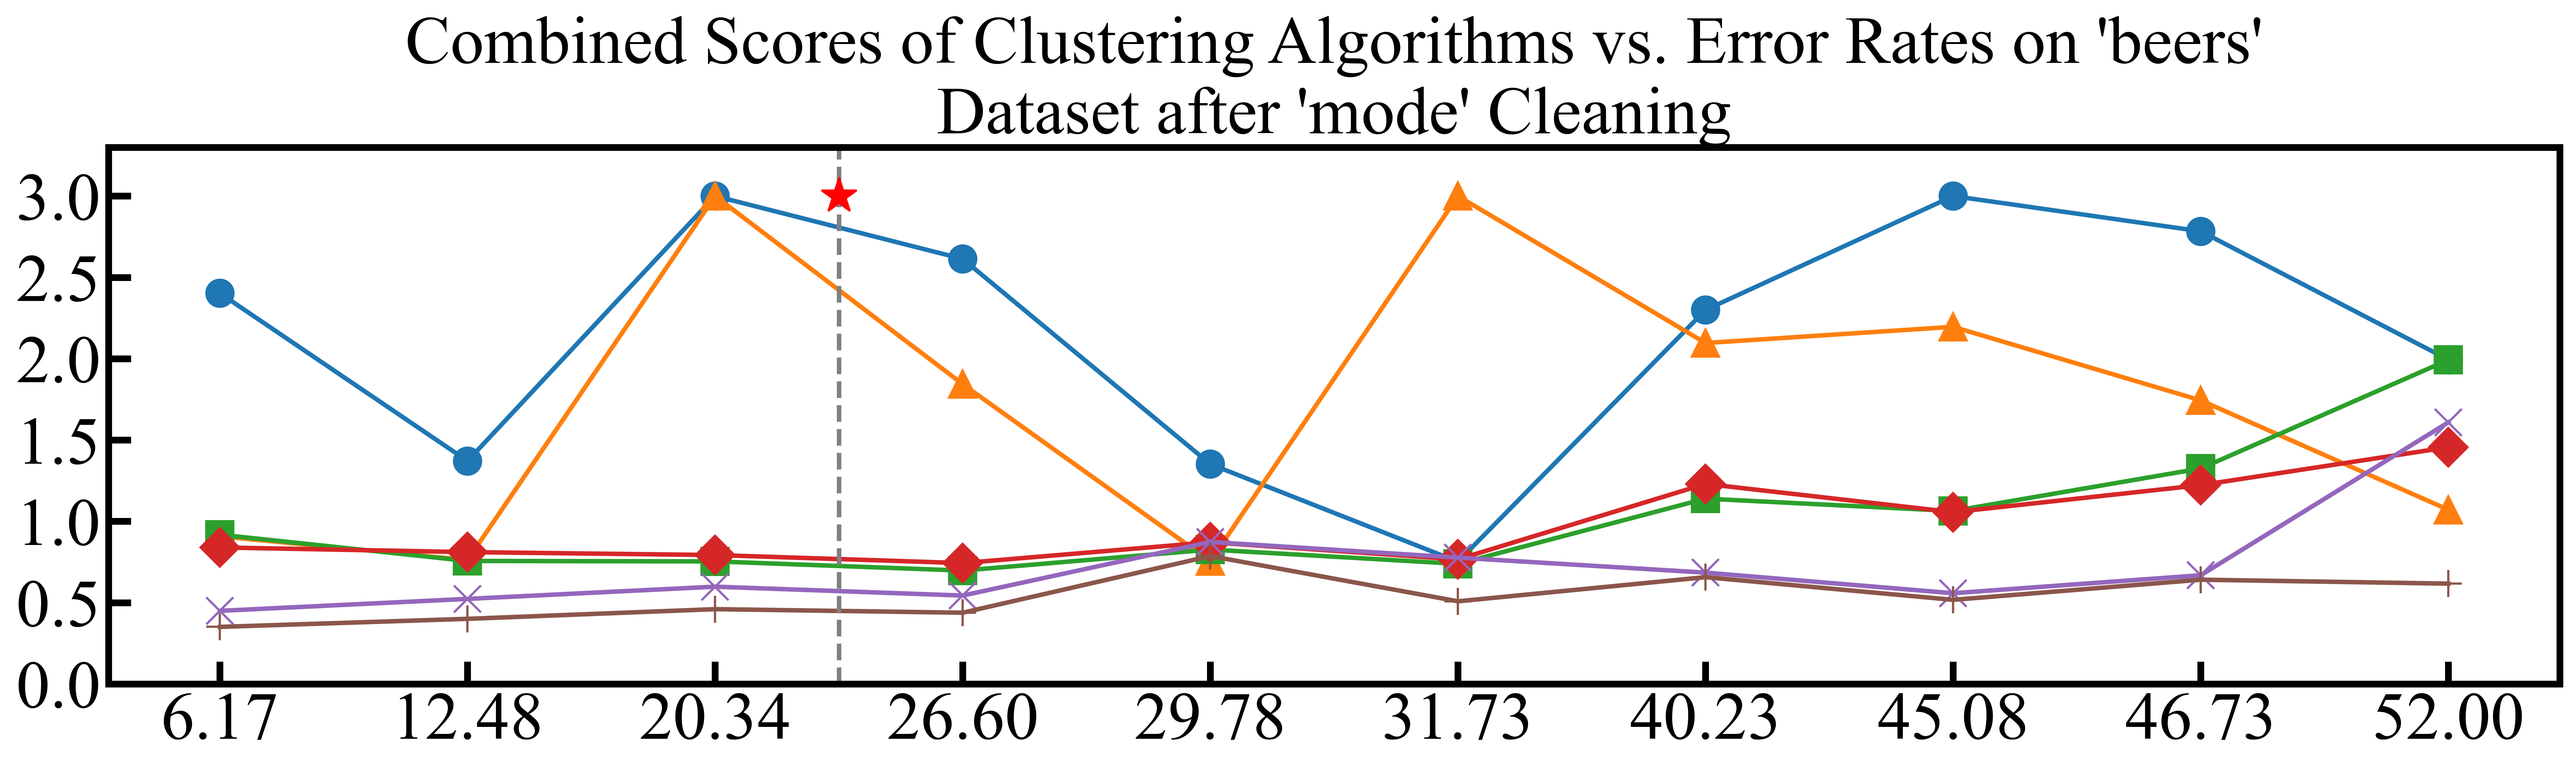
\includegraphics[width=\linewidth]{figures/mode_beers_combined_scores.png}
    \caption{\textit{mode}, Beers}
    \label{fig:mode_beers}
  \end{subfigure}
  \hfill
  \begin{subfigure}{0.48\linewidth}
    \centering
    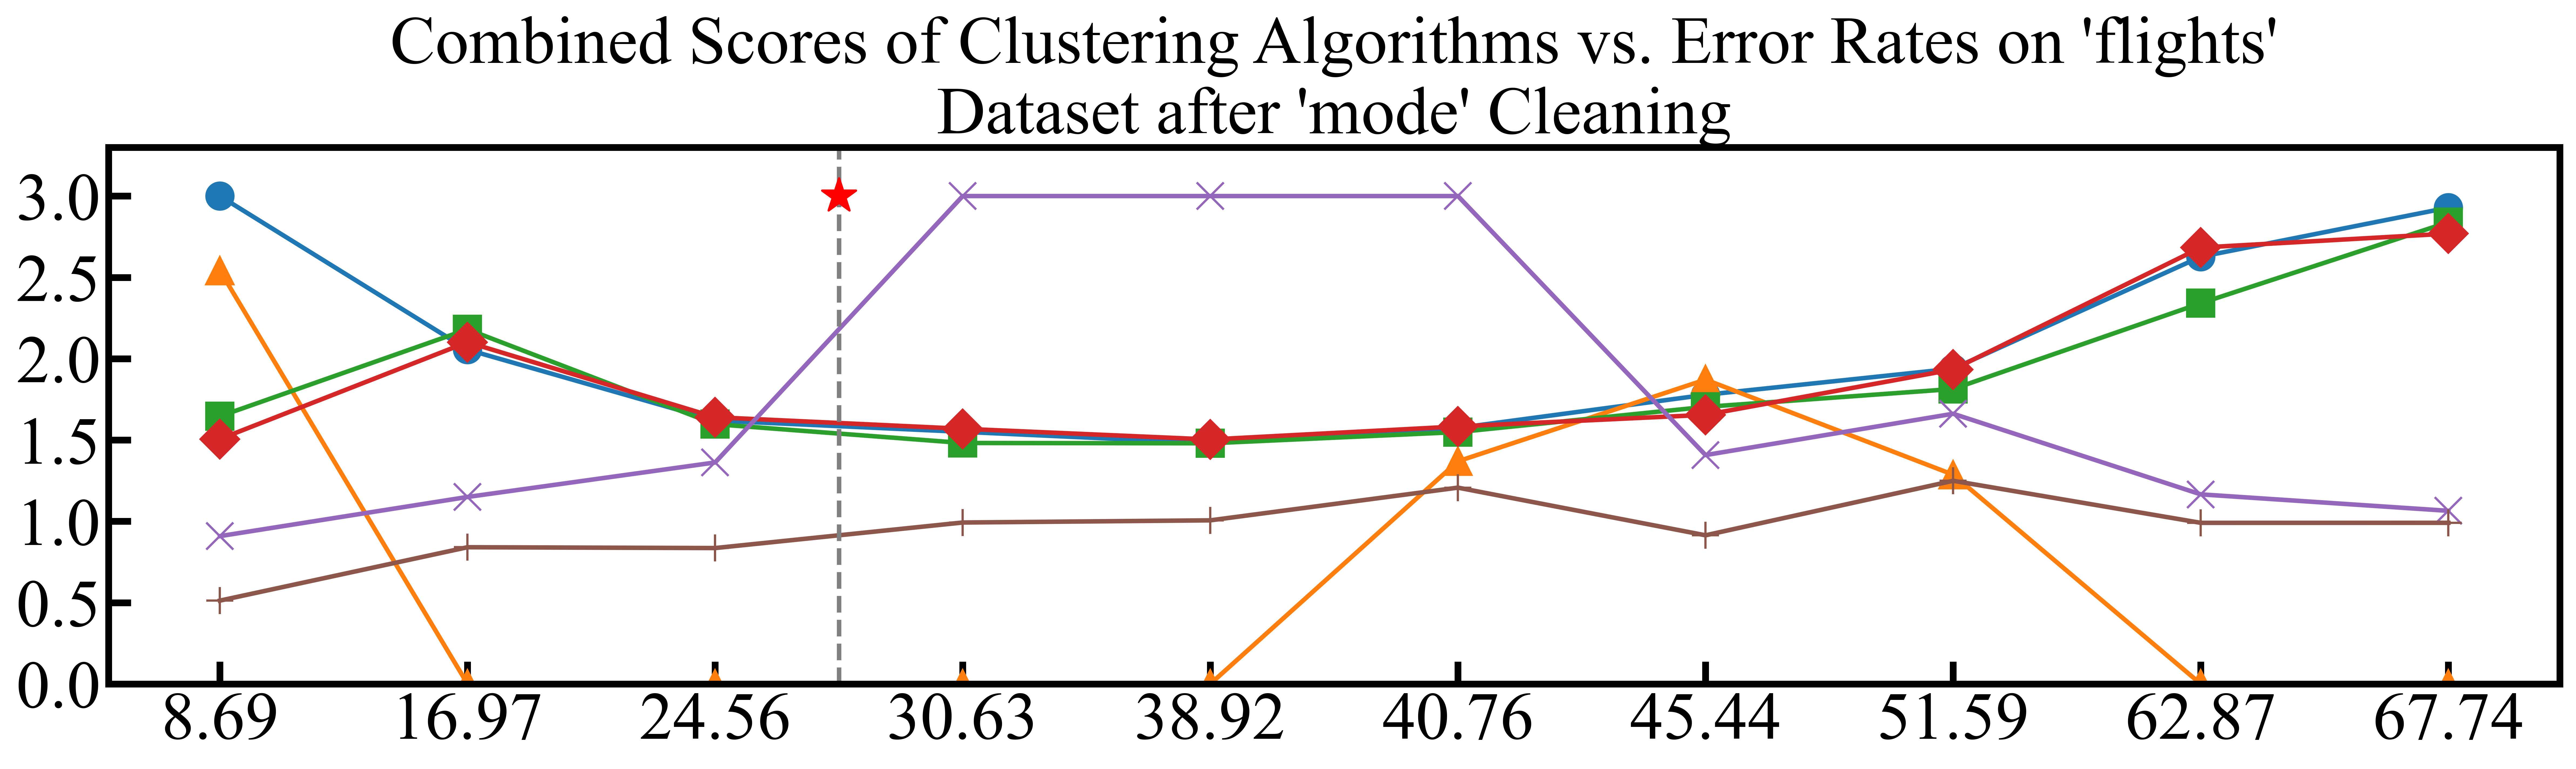
\includegraphics[width=\linewidth]{figures/mode_flights_combined_scores.png}
    \caption{\textit{mode}, Flights}
    \label{fig:mode_flights}
  \end{subfigure}

  \vspace{0.2em} % 缩小两行之间的间距

  \begin{subfigure}{0.48\linewidth}
    \centering
    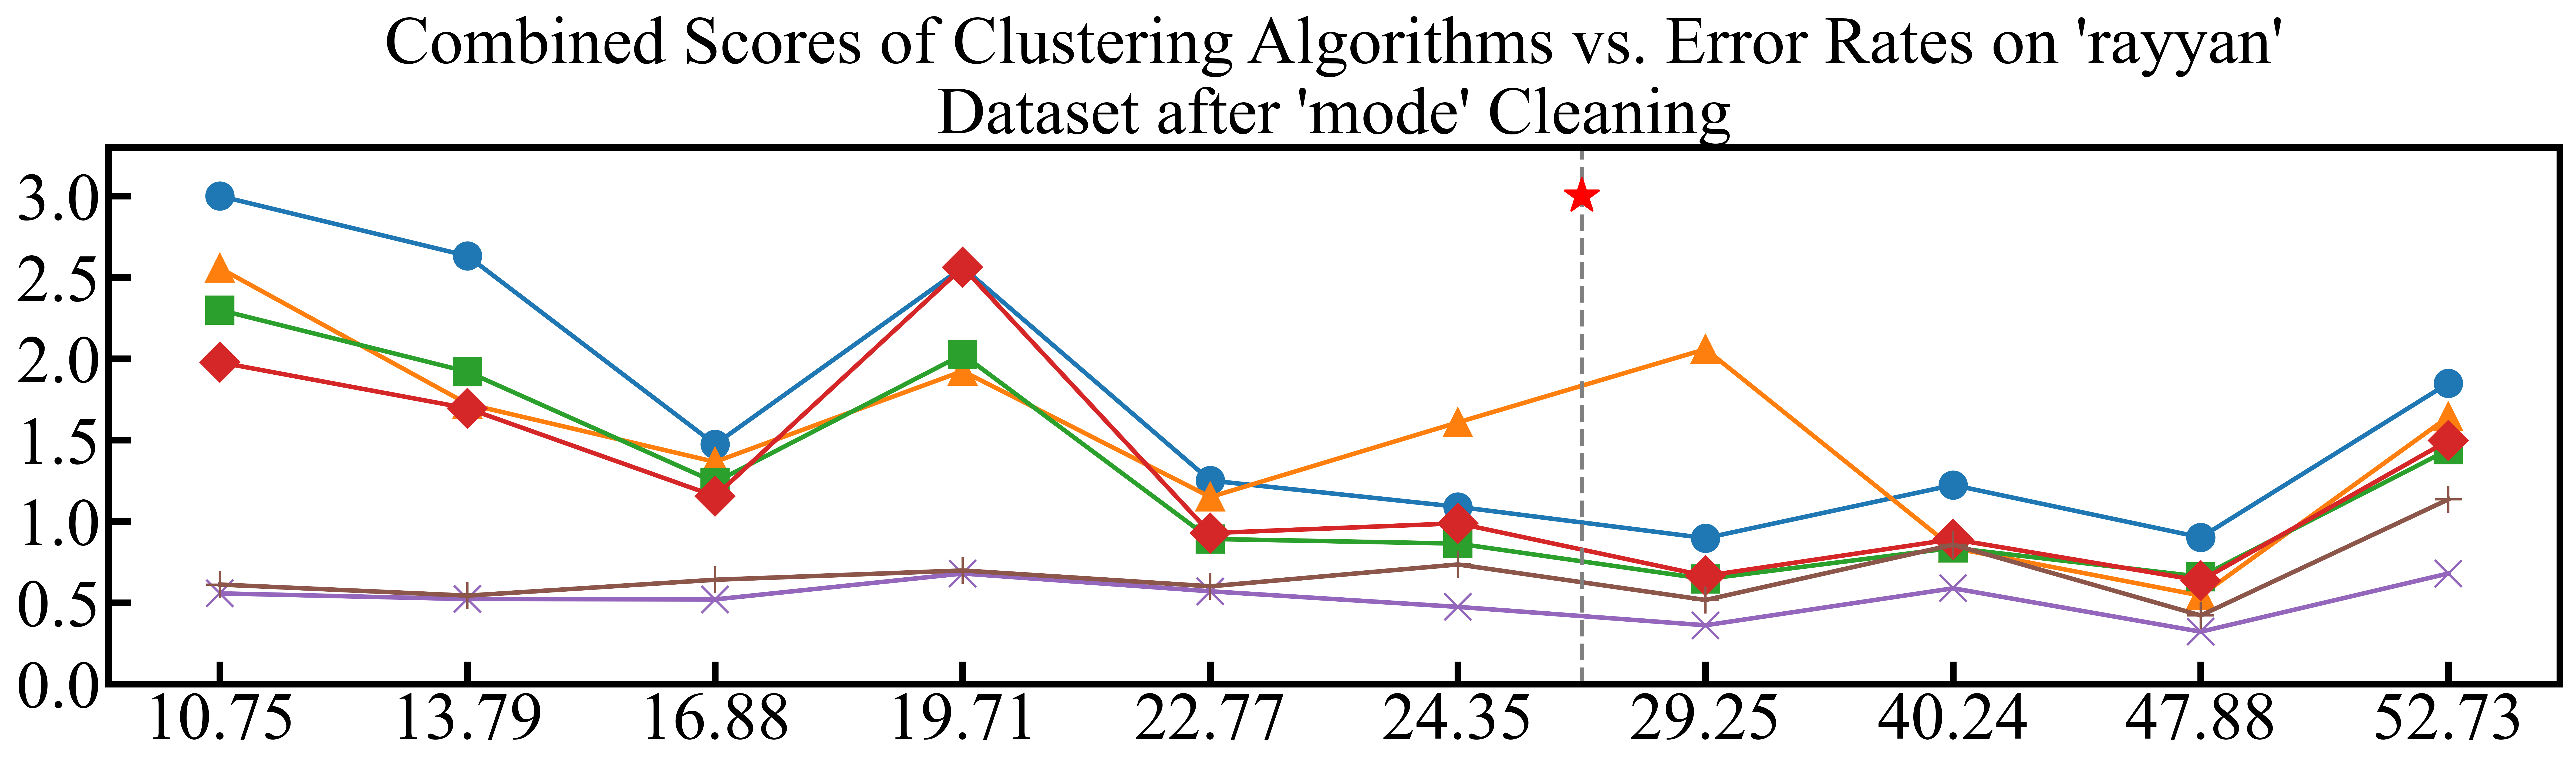
\includegraphics[width=\linewidth]{figures/mode_rayyan_combined_scores.png}
    \caption{\textit{mode}, Rayyan}
    \label{fig:mode_rayyan}
  \end{subfigure}
  \hfill
  \begin{subfigure}{0.48\linewidth}
    \centering
    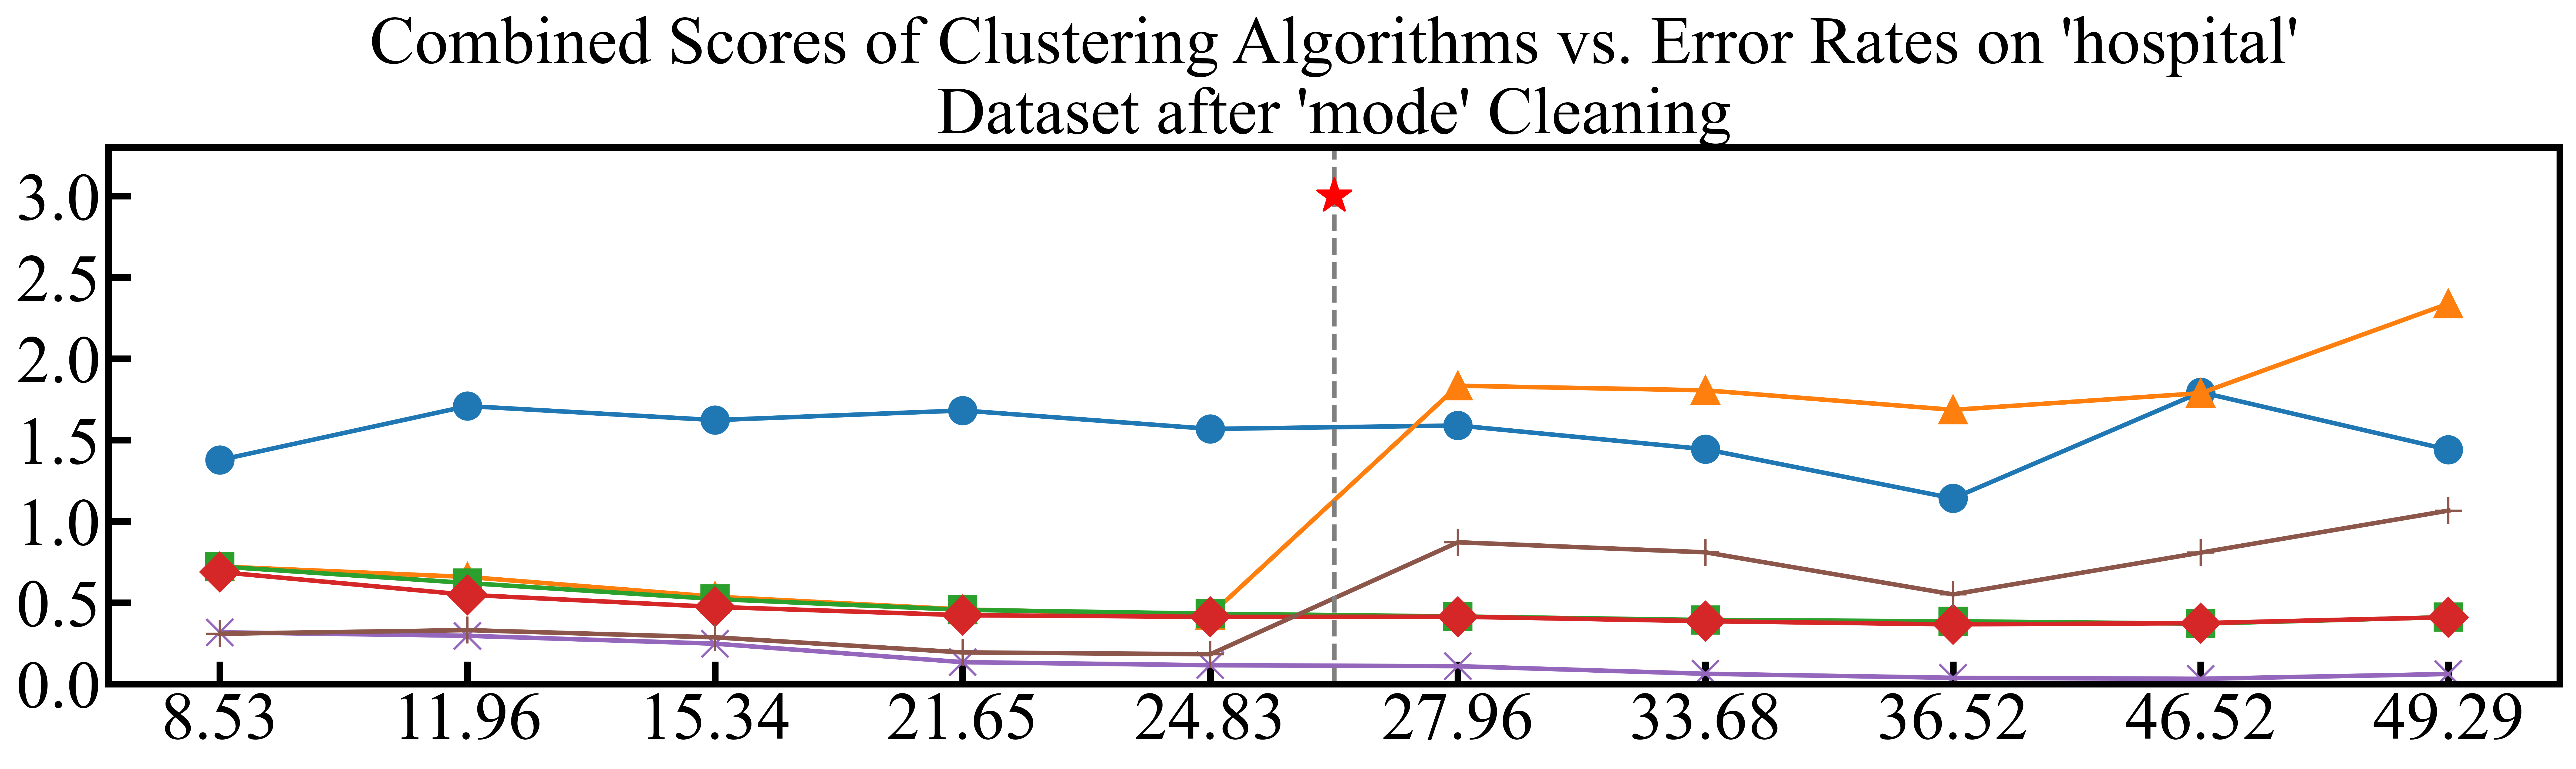
\includegraphics[width=\linewidth]{figures/mode_hospital_combined_scores.png}
    \caption{\textit{mode}, Hospital}
    \label{fig:mode_hospital}
  \end{subfigure}

  \vspace{0.2em} % 适当减少两行之间的间距

  % 第二行:Raha-Baran 清洗
  \begin{subfigure}{0.48\linewidth}
    \centering
    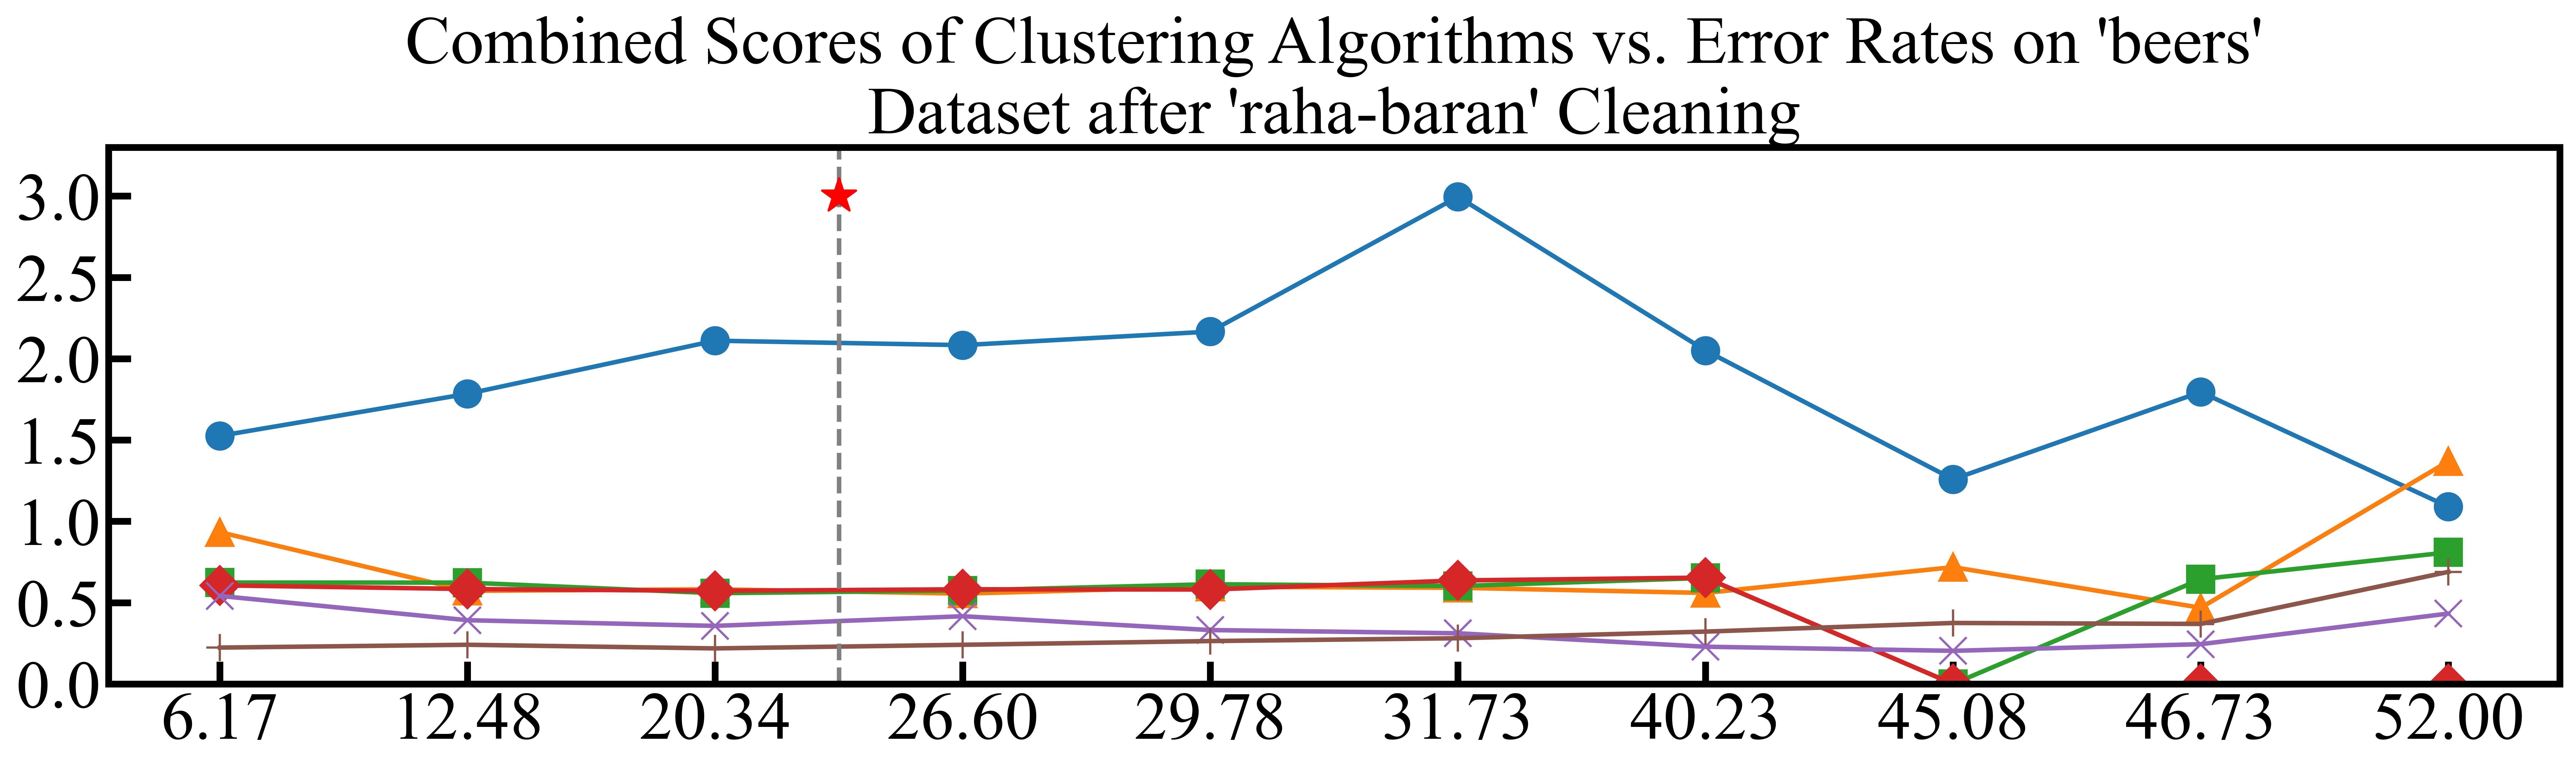
\includegraphics[width=\linewidth]{figures/raha-baran_beers_combined_scores.png}
    \caption{\textit{Raha-Baran}, Beers}
    \label{fig:raha_baran_beers}
  \end{subfigure}
  \hfill
  \begin{subfigure}{0.48\linewidth}
    \centering
    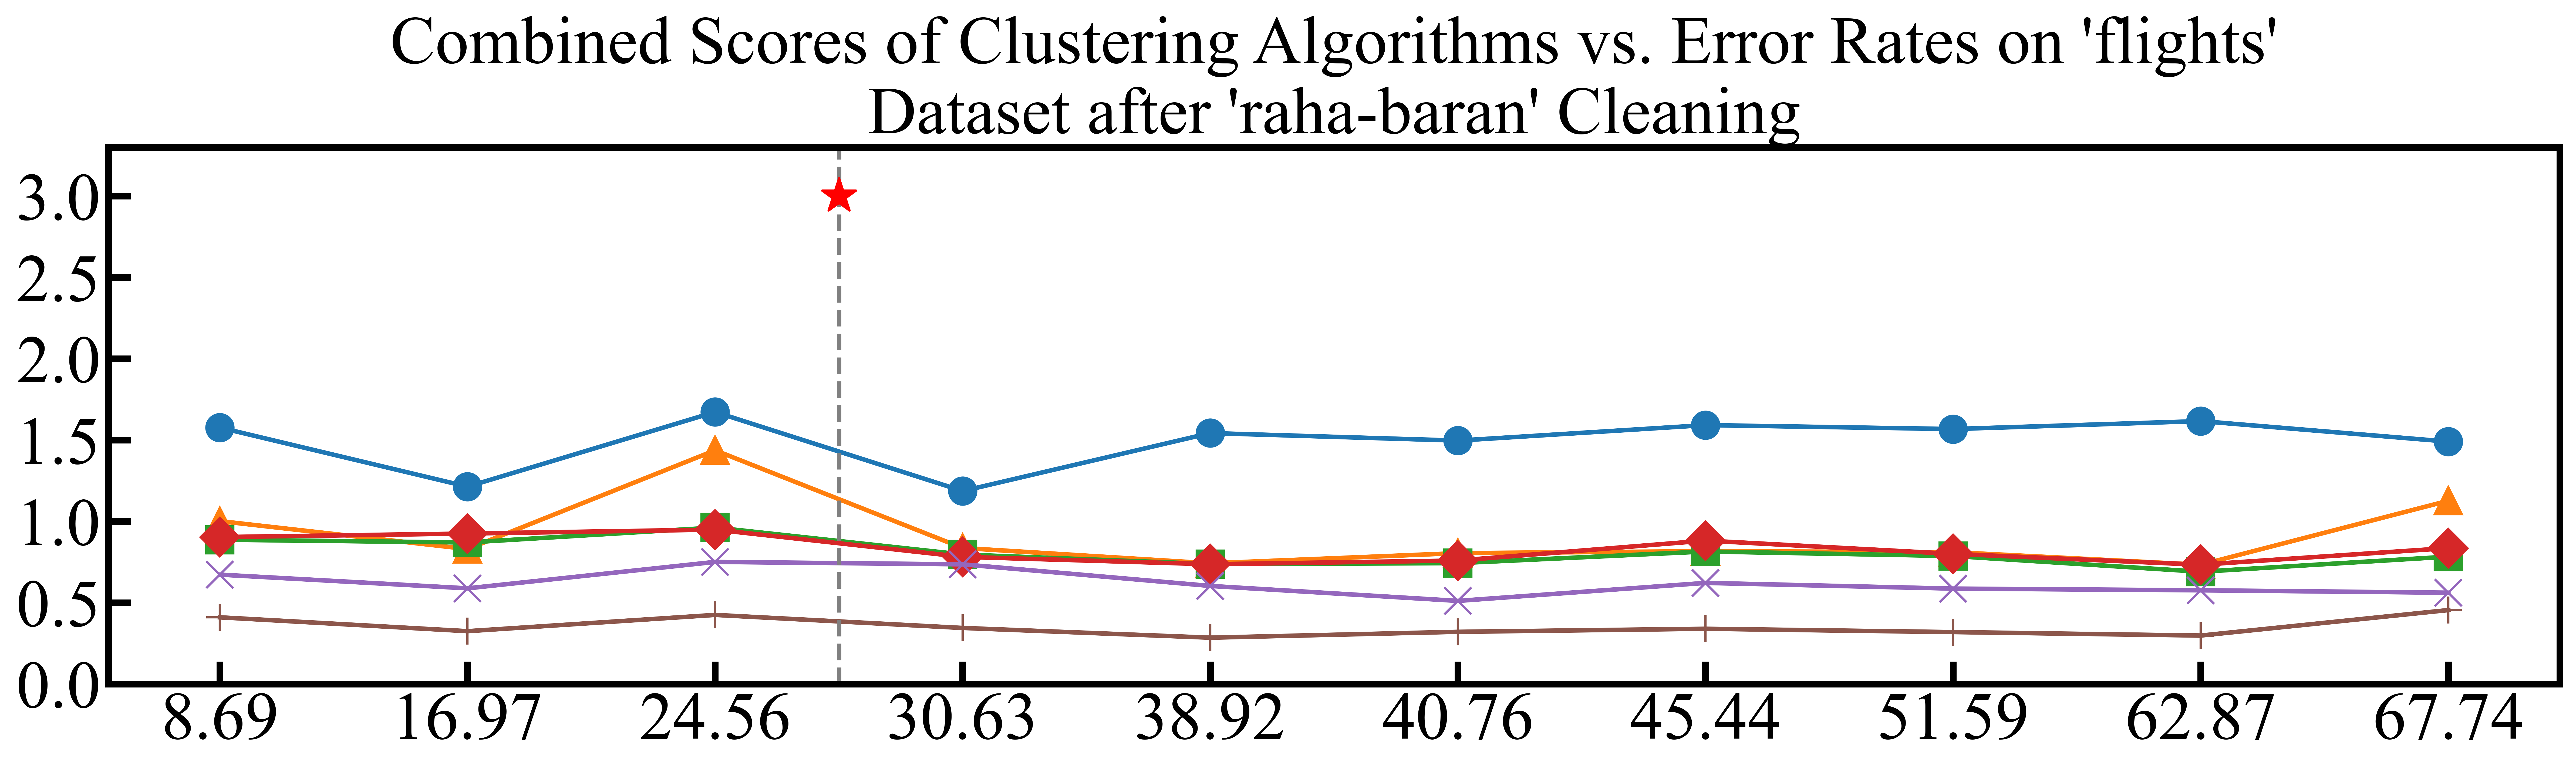
\includegraphics[width=\linewidth]{figures/raha-baran_flights_combined_scores.png}
    \caption{\textit{Raha-Baran}, Flights}
    \label{fig:raha_baran_flights}
  \end{subfigure}

  \vspace{0.2em} % 继续缩小行距

  \begin{subfigure}{0.48\linewidth}
    \centering
    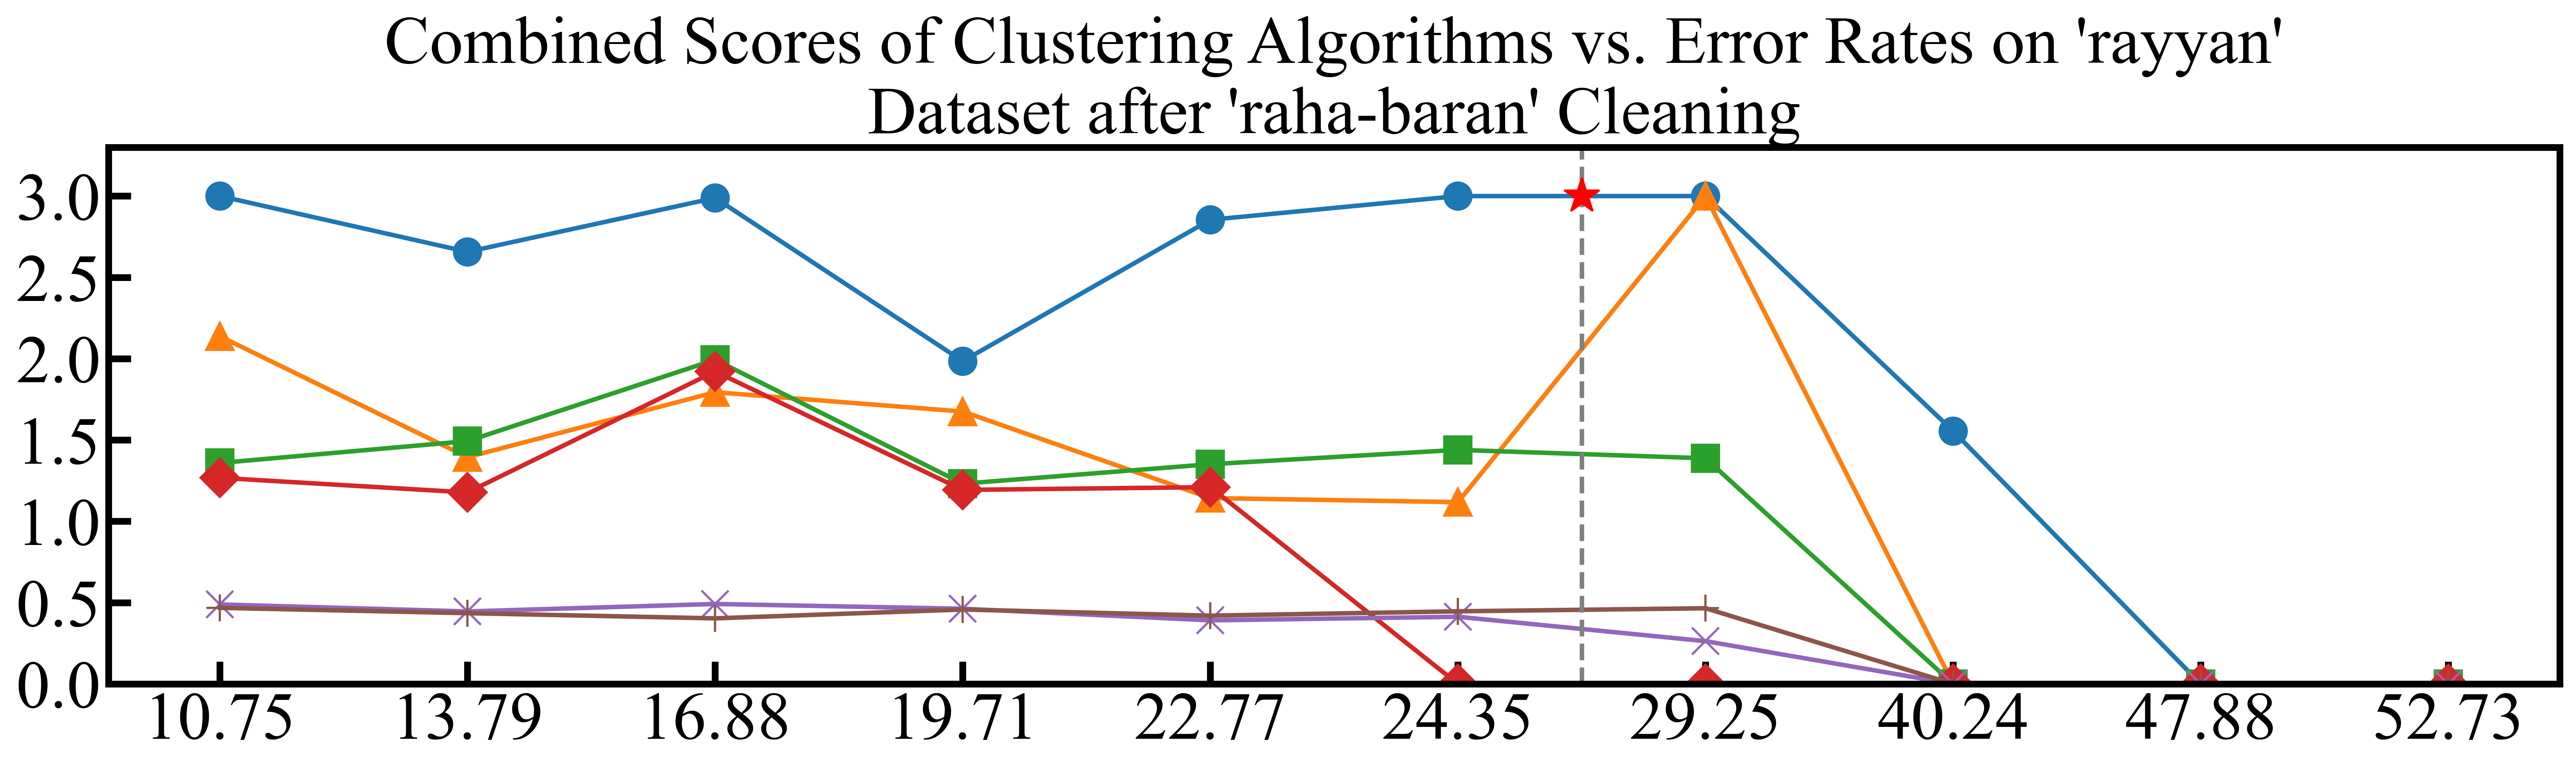
\includegraphics[width=\linewidth]{figures/raha-baran_rayyan_combined_scores.png}
    \caption{\textit{Raha-Baran}, Rayyan}
    \label{fig:raha_baran_rayyan}
  \end{subfigure}
  \hfill
  \begin{subfigure}{0.48\linewidth}
    \centering
    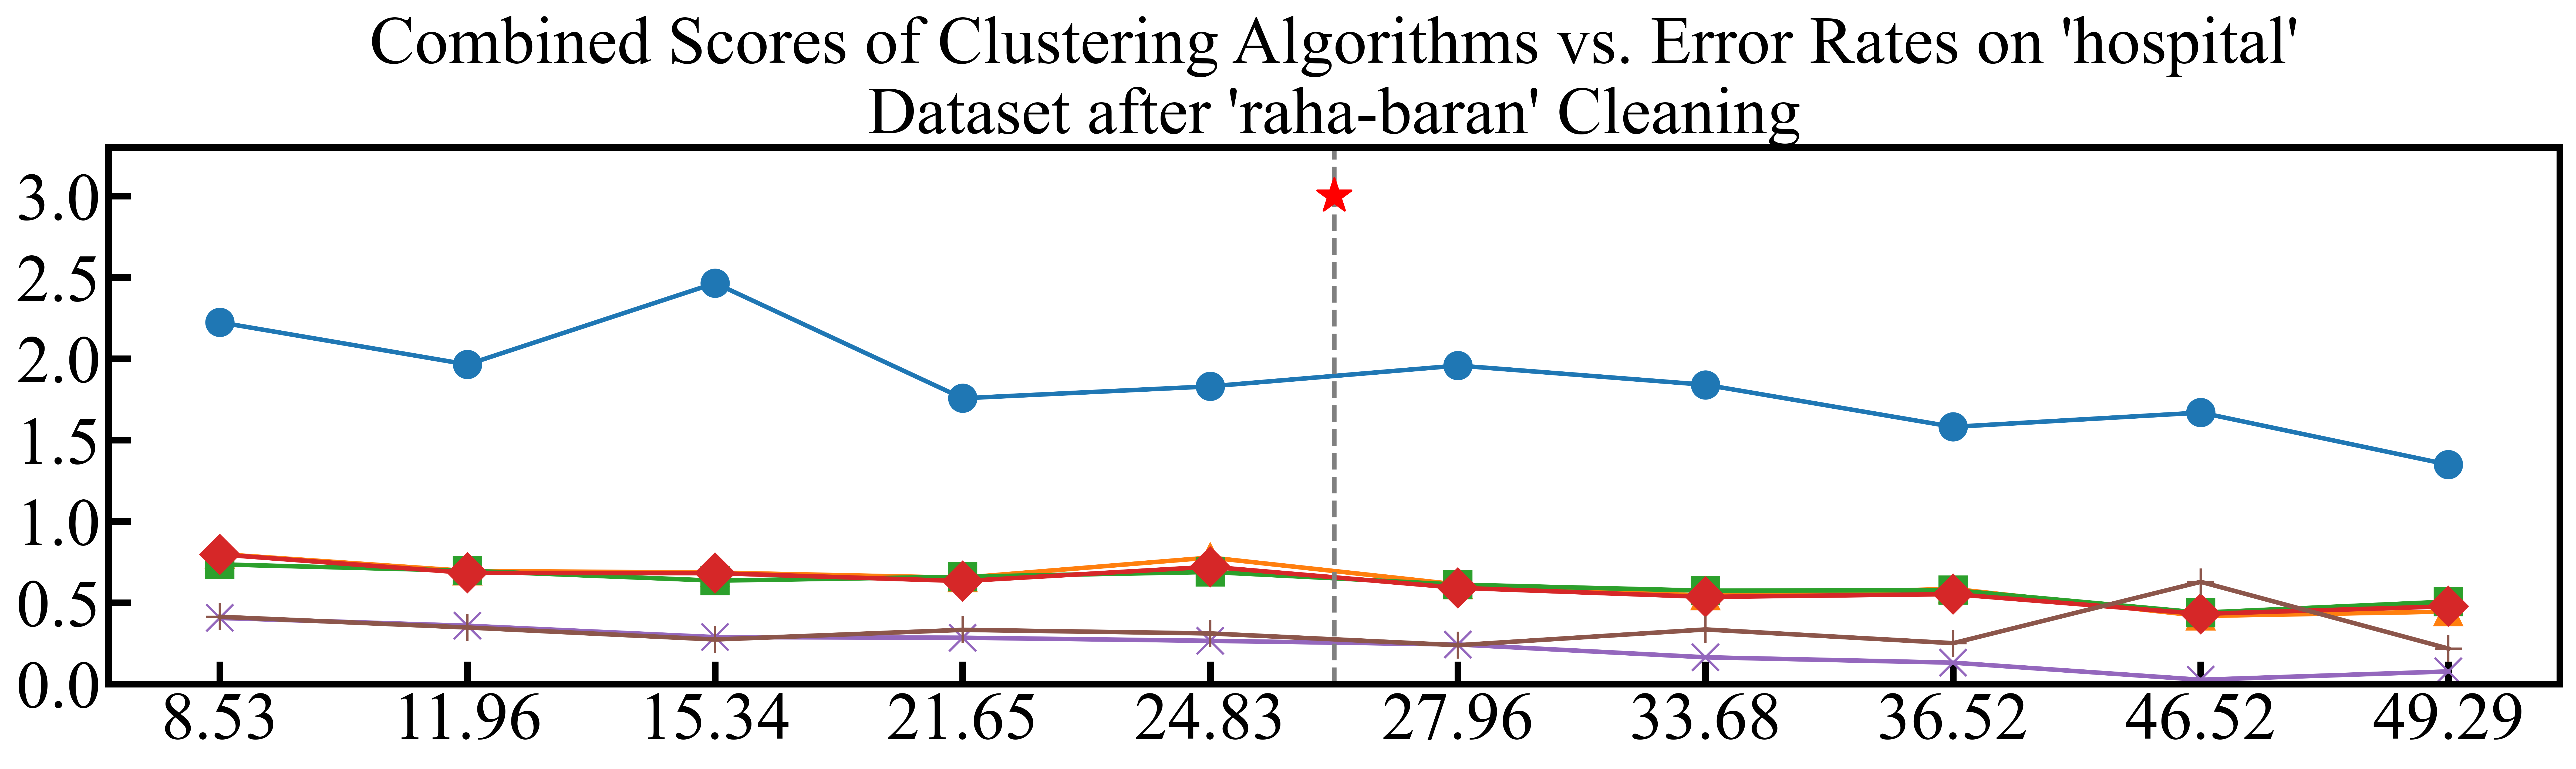
\includegraphics[width=\linewidth]{figures/raha-baran_hospital_combined_scores.png}
    \caption{\textit{Raha-Baran}, Hospital}
    \label{fig:raha_baran_hospital}
  \end{subfigure}

  \caption{不同数据集在不同错误率条件下的聚类算法综合得分变化趋势}
  \label{fig:all_combined_scores}
\end{figure}

\noindent

通过综合比对上述不同数据集在 mode 与 Raha-Baran 清洗下,各聚类算法随错误率变化的表现,可以得到以下几条规律性结论:

\begin{enumerate}
    \item \textbf{错误率升高易出现“极端爆分”或“收敛失败”,精细化清洗可缓解但不能完全避免} \\
    当错误率中高时,mode 清洗下的 HC、DBSCAN、AP 更易出现高达 3.00 的极端得分或直接收敛到 0.00。使用 Raha-Baran 虽然减少了此类“爆分”现象,但在个别极端场景下,KMeans、GMM 或 AP 仍可能无法正常聚类,导致分数骤降至 0.0。

    \item \textbf{聚类算法对错误率的敏感度差异明显,HC/DBSCAN 波动大,KMeans/GMM/OPTICS 相对平稳} \\
    层次聚类(HC)与密度聚类(DBSCAN)对噪声和超参数敏感度最高,最易在错误率升高后出现大幅波动或极端值。相比之下,KMeans 与 GMM 在大多错误率区间分数处于中等水平,不常爆分但也可能在高错误率时收敛失败;OPTICS 波动相对较小,但平均得分不高。

    \item \textbf{“mode” 与 “Raha-Baran” 的差异在高错误率下尤为突出} \\
    低或中等错误率下,两种清洗方法整体表现差异不大;但一旦错误率升至 30\% 以上,mode 更易触发少数算法的极端波动或收敛异常,而 Raha-Baran 虽也会出现偶发失效,却在多数场景保持了中等或较平稳的分数,展现出对高错误率的相对鲁棒性。
\end{enumerate}

\noindent
综上所述,随着错误率的持续升高,数据质量对聚类算法的影响呈显著放大趋势。尽管使用更精细的清洗方法(如 Raha-Baran)能够降低极端结果出现的概率,但在高噪声场景下仍有可能出现算法收敛失败。为更全面地评估不同清洗-聚类组合在各种数据集上的整体性能,我们将进一步从更多指标对策略的表现进行综合比较。

\paragraph{(3) 基于多指标的综合性能分析}
图~\ref{fig:alg_comb_metrics} 以 5 张柱状图展示了 18 种清洗-聚类组合策略在不同聚类评估指标下的整体表现,横轴为算法组合,纵轴为相应指标数值,评估指标包括:
\begin{itemize}
    \item \textbf{Average Score (\%)}:算法组合在所有实验场景中的平均得分百分比(0\%--150\%),反映其总体性能;
    \item \textbf{Average Combined Score}:综合分数均值(0--2),度量簇的紧致性与分离度的平衡;
    \item \textbf{Standard Deviation of Percentage Score}:得分百分比的标准差,表示不同场景间的波动大小;
    \item \textbf{Standard Deviation of Combined Score}:综合分数的标准差,用于评估算法在多场景下的一致性;
    \item \textbf{Average Deviation from Reference (100\%)}:相对于基准方案(100\%)的平均偏离程度,数值越小表示越接近基准。
\end{itemize}

此外,图~\ref{fig:alg_comb_metrics_low} 在上述基础上选取错误率低于 25\% 的数据,聚焦分析非极端噪声条件下各组合的聚类性能与稳定性,直观对比各方法在低错误率场景下的差异。以下是从这两类图表中得出的主要结论与启示:

\begin{figure}[htbp]
    \centering
    \setlength{\abovecaptionskip}{5pt}  % 增加标题与图片之间的间距
    \setlength{\belowcaptionskip}{5pt}  % 增加标题与正文之间的间距

    % 第一张图(单独占一行)
    \begin{subfigure}{1.0\linewidth}  % 增大宽度
        \centering
        
\includegraphics[width=\linewidth]{figures/alg_comb_metrics.png}
        \caption{18 种清洗-聚类组合在不同聚类评估指标上的综合表现}
        \label{fig:alg_comb_metrics}
    \end{subfigure}

    \vspace{1em}  % 增加两张图之间的间距

    % 第二张图(单独占一行)
    \begin{subfigure}{1.0\linewidth}  % 增大宽度
        \centering
        
\includegraphics[width=\linewidth]{figures/alg_comb_metrics_low.png}
        \caption{错误率低于 25\% 条件下,各算法组合的聚类性能与稳定性}
        \label{fig:alg_comb_metrics_low}
    \end{subfigure}

    \caption{聚类算法组合在不同条件下的评估指标比较}
    \label{fig:alg_comb_metrics_comparison}
\end{figure}

\subparagraph{全局方案表现与离散度分析}
图~\ref{fig:alg_comb_metrics} 将所有数据集(含不同错误率)的结果归纳,便于从全局角度评估各方案的稳定性与适应性。可以看到:
\begin{itemize}
    \item \textbf{高均值+高方差的“爆分”组合}:例如 mode + DBSCAN 组合虽然平均分高达 147\%,却伴随多达 481.75 的标准差 ,说明其在数值特征为主、规模较大的数据(如 \textit{flights, beers})上易发生极端聚类效果,在实际使用中需谨慎。
    \item \textbf{Raha-Baran + HC 和 mode + HC 整体分数高且方差相对适中}:  mode + HC 约 101.53\%,标准差 64.62; Raha-Baran + HC 约 90.03\%,标准差 34.80,说明层次聚类在多场景下保持稳定,Raha-Baran 在处理语义或规则错误(如 \textit{hospital, rayyan})时尤为有效。
    \item \textbf{其余组合多集中在 30\%--70\% 区间}:如 Raha-Baran + OPTICS 均值仅 16.75\%,在当前参数设置与数据特征下并未取得良好协同,凸显密度聚类方法在高维或高噪声环境中对参数匹配的依赖度。
\end{itemize}
总体而言,DBSCAN/OPTICS 虽具潜力但波动大,HC 与合适的清洗策略(Mode 或 Raha-Baran)通常兼具更高均值和更低方差。

\subparagraph{低错误率情形下的表现}
在图~\ref{fig:alg_comb_metrics_low} 中仅保留错误率低于 25\% 的数据,用以检验数据质量较佳时的聚类性能及稳定性。结果表明:
\begin{itemize}
    \item \textbf{Mode + HC 均值约 100.14\%},但标准差 74.20:在低错误率场景下,简单填补能够较好保留数据分布,HC 则通过合适的层次切分实现高分。然而,在高维或噪声分布不均的情况下,其表现仍可能出现较大波动。
    \item \textbf{Raha-Baran + HC 稳定性更佳}:均值约 91.04\%,标准差降至 20.04,显示对具备语义或知识库错误的数据集(如 \textit{hospital, rayyan})而言,精细化修复能显著减少噪声干扰,HC 则在较低错误率下持续逼近或略超基准。
    \item \textbf{其余组合受益有限}:如 mode + GMM、mode + KMeans 等平均分多介于 50\%--60\%,虽较全局时略有提升,但在面向 11--20 个特征的中等维度数据时仍不具明显优势。
\end{itemize}

\subsubsection{综合分析与实践建议}
结合上述实验结果和多种清洗与聚类算法的表现,针对不同规模、特征类型及错误率水平的数据集,提出以下建议来指导清洗与聚类策略的选择:

\begin{itemize}
    \item \textbf{小至中规模数据集、高维/多元特征且可能存在语义错误}:
    优先选择 Raha-Baran + HC 组合。Raha-Baran 的上下文修复能力能够有效处理复杂语义错误,而 HC(层次聚类)的分层聚类特性适合高维、多特征数据。若错误率较高,需进一步结合更先进的修复策略,或通过特征选择与降维手段减少特征复杂性。

    \item \textbf{中至大规模数据集、以数值型特征为主、对内部指标最优化有较强需求}:
    考虑使用 mode + HC 或 mode + DBSCAN。简单填补策略(Mode)在数值型数据上的效率较高,而 HC 和 DBSCAN 均能对中大规模数据集进行合理划分,但需谨慎对待 mode + DBSCAN 的高方差风险。若应用场景要求聚类结果与基准结构更贴近且解释性更强,应该选择更稳健的组合(如 mode + HC 或 mode + KMeans)。

    \item \textbf{强噪声分布、不规则簇形状的数据集}:
    可使用 DBSCAN 或 OPTICS 等密度聚类方法。这些方法在处理不规则簇形状和高噪声数据时具有明显优势。密度聚类方法对超参数(如 $\varepsilon$ 和 $\xi$)敏感,因此需要针对不同错误率和分布特征进行精细化超参数调优,以避免出现极端分割(过多单点簇)或过度聚合的情况。自动调优框架(如 Optuna)在此类场景中尤为重要。
\end{itemize}

这些建议为后续应用中选择清洗-聚类方法提供了可行的依据,也为在高噪声及多样化数据环境中平衡聚类质量与可解释性指出了明确方向。

\subsection{自动化聚类模型评估实验}
\label{sec:automl_exp}
本节基于第~\ref{sec:large_scale_exp} 节的大规模对比实验,利用先验数据集训练多标签分类器,并测试自动化优化管线在部分数据集上的性能(见表~\ref{tab:autoML_res})。实验旨在重点评估第~\ref{sec:autoML} 节提出的优化管线在缩减搜索空间的同时,是否能保持较高的聚类质量,主要考察\textbf{损失率} \(\eta(D)\) 和\textbf{综合加速比} \(\mathcal{A}(D)\) 两项关键指标。实验结果表明,该方法能够有效减少无效组合的尝试,使评估时间平均减少 5\textasciitilde10 倍,而聚类得分的损失率仅在 1.9\%\textasciitilde3.1\%之间。

\begin{table}[htbp]
\centering
\begin{tabular}{lcccc}
\toprule
\textbf{数据集} & \textbf{全量搜索耗时 (s)} & \textbf{自动化耗时 (s)} & \textbf{加速比} & \textbf{损失率 (\%)} \\
\midrule
Beers & 10.5 & 2.4 & 4.4 & 3.1 \\
Flights & 18.2 & 2.1 & 8.7 & 2.8 \\
Hospital & 25.0 & 3.2 & 7.8 & 1.9 \\
\bottomrule
\end{tabular}
\caption{自动化聚类优化管线 vs. 全量搜索}
\label{tab:autoML_res}
\end{table}

\noindent
从表~\ref{tab:autoML_res} 可以看出,自动化方法能够大幅缩减计算成本,尤其在大规模数据集(如 \textit{flights})上,搜索时间缩短至全量搜索的 1/8,而得分损失保持在 3\%以内,表明该方法在保持较高聚类质量的前提下,实现了显著的搜索加速。其中:
\begin{itemize}
    \item 低损失率:\texttt{Hospital} 数据集的损失率仅 1.9\%,说明自动化管线对高维、多特征数据依然保持较好性能;
    \item 高加速比:在 \texttt{Flights} 数据集上,加速比达到 8.7 倍,适用于计算成本敏感的应用场景;
    \item 稳定性:所有数据集上的损失率均控制在 3.1\% 以下,显示该方法具有较好的泛化能力。
\end{itemize}

\noindent
综上所述,自动化聚类优化管线在大幅降低计算开销的同时,仅牺牲极小的聚类质量,证明了其在高效聚类任务中的实用价值。 

%---------------------------------
% 第六章:结论
%---------------------------------

\section{结论}
\label{sec:conclusion}

本文针对数据质量问题(错误值、缺失值、噪声)对聚类任务的影响,提出了一种\textbf{清洗-聚类协同优化}方法,并基于\textbf{自动化管线模型}提升搜索效率。通过在 40 个公开数据集上的实验,评估了三种清洗策略(Mode 填补、Raha-Baran 修复、GroundTruth 基准)与六种聚类算法(K-Means、DBSCAN、OPTICS、层次聚类、GMM、AffinityPropagation)的组合表现。主要结论如下:

\begin{enumerate}
    \item \textbf{数据清洗与聚类算法的协同优化至关重要:}
    清洗方法显著影响聚类效果,不同策略适用于不同数据特征。Raha-Baran + HC 在高维、语义约束数据上表现稳健,而 Mode + DBSCAN 在低维数值型数据中可能产生极端得分,但与真实结构偏离较大。

    \item \textbf{自动化管线显著提升搜索效率:}  
    通过多标签学习建模“数据特征—最优策略”映射,可有效缩小搜索空间,在损失率控制在 3\% 以内的同时,实现 5\textasciitilde10 倍加速,验证了该方法的实用性。

    \item \textbf{数据特征与错误率决定最优策略选择:}  
    数据规模、特征多样性、错误率等因素决定了最优清洗-聚类组合。稳健性优先时可选择 Raha-Baran + HC 或 Mode + KMeans,而密度聚类(DBSCAN、OPTICS)对超参数敏感,需谨慎调优。
\end{enumerate}

\paragraph{未来工作方向}  
后续研究可进一步优化以下方面:
\begin{itemize}
    \item \textbf{复杂数据清洗:} 结合知识图谱、联合学习等方法处理跨属性错误与语义冲突。
    \item \textbf{增量式聚类优化:} 研究流式数据场景下的动态策略推荐与自适应管线调整。
    \item \textbf{超参数智能调优:} 利用贝叶斯优化、遗传算法等提升密度聚类的稳定性,并增强可解释性分析。
\end{itemize}

综上,本文在\textbf{数据清洗、聚类优化、自动化管线}三方面提供了系统性探索,验证了协同优化的有效性,并为高噪声、大规模数据场景下的聚类任务提供了实用解决方案。

%---------------------------------
% 参考文献(可选)
%---------------------------------
\bibliographystyle{IEEEtran}
\bibliography{references}

\end{document}
